\documentclass[11pt,a4paper]{article}

% A shorter, LessWrong-facing edition. The full research draft remains main.tex.
\usepackage[left=1in,right=1in,top=0.9in,bottom=1in]{geometry}
\usepackage[T1]{fontenc}
\usepackage[utf8]{inputenc}
\usepackage{palatino}
\usepackage{microtype}
\usepackage[all]{nowidow}
\global\hyphenpenalty=700
\setlength{\parindent}{0pt}
\setlength{\parskip}{0.62em}
\raggedbottom

\usepackage[numbers,round]{natbib}
\bibliographystyle{naturemag}
\usepackage[table,xcdraw]{xcolor}
\usepackage{url}
\usepackage{hyperref}
\hypersetup{
  colorlinks=true,
  linkcolor={red!45!black},
  citecolor={blue!45!black},
  urlcolor={blue!70!black},
  pdftitle={Predicting Learned Goals: ForkWorld}
}

\usepackage{graphicx}
\graphicspath{{figures/}}
\usepackage{booktabs}
\usepackage{tabularx}
\usepackage{longtable}
\usepackage{adjustbox}
\usepackage{pdflscape}
\usepackage{placeins}
\usepackage{float}
\renewcommand{\topfraction}{0.92}
\renewcommand{\bottomfraction}{0.85}
\renewcommand{\textfraction}{0.08}
\renewcommand{\floatpagefraction}{0.78}
\setcounter{topnumber}{2}
\setcounter{bottomnumber}{1}
\setcounter{totalnumber}{3}
\usepackage[font=small,labelfont=bf]{caption}
\usepackage{amsmath}
\usepackage{amssymb}
\usepackage{enumitem}

\definecolor{intended}{HTML}{2673B8}
\definecolor{proxy}{HTML}{D55E00}
\definecolor{evidence}{HTML}{009E73}
\definecolor{softgray}{HTML}{F2F4F7}
\definecolor{ink}{HTML}{17212B}

\newcommand{\rhoY}{\rho_Y}
\newcommand{\rhoP}{\rho_P}
\newcommand{\Forkworld}{\textsc{Forkworld}}
\newcommand{\CI}{\textsc{ci}}
\newcommand{\fig}[1]{Fig.~\ref{#1}}

\newenvironment{takeaway}{%
  \begin{quote}\small\color{ink}\noindent\textbf{Takeaway.}\ 
}{%
  \end{quote}
}

\makeatletter
\renewenvironment{abstract}{%
  \vspace{-10pt}%
  \centerline{\large\bfseries TL;DR}%
  \setlength{\leftmargini}{30pt}%
  \begin{quote}\small
}{%
  \par\end{quote}\vskip 1ex
}
\makeatother

\title{\textbf{Predicting Learned Goals}\\[-1mm]
\large ForkWorld}
\author{}
\date{}

\begin{document}

\maketitle

\begin{abstract}
A model can perform perfectly on the distribution used to train and validate it while relying entirely on the wrong rule. We built \Forkworld{} to make this ambiguity measurable. A small neural network chooses between two destinations using an intended rule and one or more easier proxies; we then evaluate it only where those rules disagree and intervene on the candidate inputs. In this post, ``motivation'' means the rule that causally controls behavior under those disagreement interventions. It does not mean a subjective desire or a uniquely identified internal utility function.

Across the experiments, models usually learned easy proxies before harder exact rules. Dataset size alone did not predict whether the intended rule would take control; counterexamples from varied contexts and examples where several shortcuts failed together were more informative. Separate exact-only models often decoded the intended rule perfectly even when matched competition models remained completely proxy-controlled. Boolean rules with the same number of inputs also competed differently, so neither decodability nor any single measure of simplicity predicted the winner. Allowing more parameters to change first strengthened the proxy and sometimes later enabled the intended rule. SFT escaped one proxy trap that RL did not; fresh zero-mean noise redirected behavior instead of washing out; and presenting the same collection of examples in a different order produced different controllers. In total, the study includes 54,930 completed training runs, with statistical inference based on independent training seeds.

The models also sometimes behaved according to different rules in different contexts or shifted temporarily to another rule during training. Those patterns complicate claims about unlearning and latent goals: perfect behavioral reversal sometimes installed the inverse proxy, while scratch and compute-matched controls reproduced most of the apparent rebound. Taken together, the results suggest that behavioral control depends on which examples distinguish the candidate rules, how easy each rule is for the particular model to learn, how the rules compete during optimization, whether behavior combines several rules, and what the model learned earlier. These are results from toy models, not evidence that frontier models use the same mechanisms. They motivate concrete evaluation practices for LLM post-training and RLHF: construct cases where plausible reward-correlated rules disagree, supplement probes with causal tests, vary the order and context of training examples, and compare suspected memory effects with matched controls.
\end{abstract}

\section*{The safety problem: performance does not identify the objective}

Suppose a model receives high reward for helping users during post-training. The observed behavior may be consistent with several rules: follow the user's intent, produce answers that a reward model likes, imitate a preferred style, agree with the evaluator, or exploit some artifact correlated with approval. If these rules agree on the training distribution, high reward cannot tell us which one will govern behavior after deployment. The ambiguity becomes visible only on inputs where the candidate rules recommend different actions.

This ambiguity is the safety-relevant core of goal misgeneralization. A system can retain the capability to act competently out of distribution while selecting actions according to an unintended objective \citep{langosco2022goal,shah2022goal}. The problem is related to underspecification and shortcut learning: models with indistinguishable in-domain performance can implement different solutions and diverge under a shift \citep{damour2022underspecification,geirhos2020shortcut}. The special concern is not merely that predictions become inaccurate, but that an agent continues to act coherently while a different rule determines what it tries to accomplish.

We use ``goal'' and ``motivation'' in a deliberately operational sense. We do not infer subjective wants, a unique utility function, or an internal search process. A candidate goal is the rule that \emph{causally controls the model's choice when plausible rules disagree}. This framing is close to recent proposals to treat motivations as behavior-influencing computations selected during training \citep{mallen2025behavioral,africa2026intentions}. It also keeps separate the signal used to update a policy from the rule the resulting policy follows \citep{turner2022reward}. Unlike analyses of mesa-optimization, the experiments do not assume that the selector performs an internal search \citep{hubinger2019risks}.

\subsection*{Forkworld}

\Forkworld{} removes most of the realism in order to make goal attribution unusually clean. On each example, a selector chooses the left or right target. A frozen controller can then navigate to the selected target, so the main experiments ask which destination is chosen rather than whether the model knows how to move through a maze.

The selector sees an intended binary label $Y\in\{-1,+1\}$ through an exact code and an easy proxy $P$. The proxy agrees with the intended label with probability
\[
\Pr(P=Y)=q.
\]
In the baseline, the exact code is parity: $Y=\prod_{i=1}^{k}R_i$. No strict subset of the $k$ bits predicts $Y$, whereas the proxy can be read from one coordinate. Most training rows have $P=Y$, so either rule gives the rewarded action. On the diagnostic distribution we force $P=-Y$ and measure
\[
\rhoY=\Pr(\widehat A=Y).
\]
A score near one means that the intended rule controls the action; a score near zero means that the proxy does. We also flip $P$ or an active exact-code bit while holding the rest of an input fixed. These interventions distinguish mere agreement with a rule from causal dependence on its channel.

Most runs stop at this one-step interface: there is no spatial grid, the action is simply ``left target'' or ``right target,'' and reward is one exactly when the choice matches $Y$. The fixed-fork rollout is neither a $2\times3$ abstraction nor a large open world. It is a $7\times7$ wall grid shaped as a symmetric T corridor; both targets are seven primitive moves from the start, and only the left/right move at the central fork depends on the selected goal. A separate $9\times9$ random-obstacle environment tests whether the selected goal can drive navigation on maps used to pretrain the controller. In both environments the selector chooses a target once, then a frozen two-hidden-layer navigator emits the four cardinal grid actions. RouteWorld later adds one, two, or four learned branch choices inside larger walled mazes, but its branch logits are computed from global route signals and a stage index rather than from online maze observations or history. Exact layouts, observations, horizons, and network architectures are specified in Appendix~\ref{sec:environment-specification}.

Later experiments add a second proxy, context-dependent rules, sequential training phases, other Boolean encodings, and repeated forks in small mazes. The primary test nevertheless remains simple: when candidate explanations of training success are made to disagree, which explanation predicts and causally changes the action?

The completed dataset contains 54,010 runs from thirteen experiment families whose designs and primary analyses were fixed internally before full execution, plus 920 runs from six follow-up panels designed after earlier results had been inspected. This internal planning was not a public or timestamped preregistration. We distinguish the two groups throughout: the first tests predictions specified before the full runs, while the second investigates patterns noticed in earlier results. Engineering pilots, smoke tests, and deterministic replays are excluded from the counts and scientific analyses.

\section*{Finding 1: Perfect in-distribution results can hide complete proxy control}

An agreement example can teach the correct action without identifying why it is correct. If $P=Y$, both ``follow the proxy'' and ``compute the intended rule'' fit the row. Only the fraction $1-q$ on which they disagree supplies evidence that separates them. Meanwhile, the proxy offers an immediate loss reduction: one weight can capture most labels. Parity becomes useful only after several features are combined.

We therefore expected training to follow a characteristic path in which the model first learns the cheapest rule that predicts reward. If sufficiently informative proxy failures continue to produce errors, the model may later build the harder exact rule and transfer control to it. When those failures are absent or too weak, however, excellent performance can lock in the shortcut. This expectation is consistent with controlled studies of simplicity bias and gradient starvation, in which one predictive route suppresses learning along another \citep{shah2020pitfalls,pezeshki2021gradient}.

In the phase grid, whose design and analysis were fixed before the full runs, we varied proxy accuracy, parity degree, and network width across 2,000 runs. At $q=.99$, mean intended-rule reliance fell from 1.000 for one active bit to .117 for five-bit parity. The width-8, five-bit cell achieved 99\% in-distribution accuracy while following the proxy on every conflict input. When $q=1$, every tested model with $k\geq2$ had perfect in-distribution accuracy and complete proxy control, at every width. Feature flips confirmed this interpretation: proxy-controlled policies changed almost every decision when $P$ was flipped and almost none when an exact-code bit was flipped, while intended-controlled policies showed the reverse pattern.

In a second panel planned before the full runs, we followed 2,400 training runs through 8,192 updates and could identify acquisition order in 2,399 of them. The proxy came first in about 91\% when each training seed received equal weight, and in all 1,655 runs that eventually acquired both rules. Median acquisition occurred at 14 updates for the proxy and 279 for the intended rule. Among shorter runs, 76\% of models that first acquired the proxy later replaced it with the intended rule. Replacement was common when counterexamples were plentiful, declined as $q$ approached one, and never occurred when the proxy was perfect. \fig{fig:phase-short} places the final phase map beside these learning curves.

\begin{figure}[!t]
  \centering
  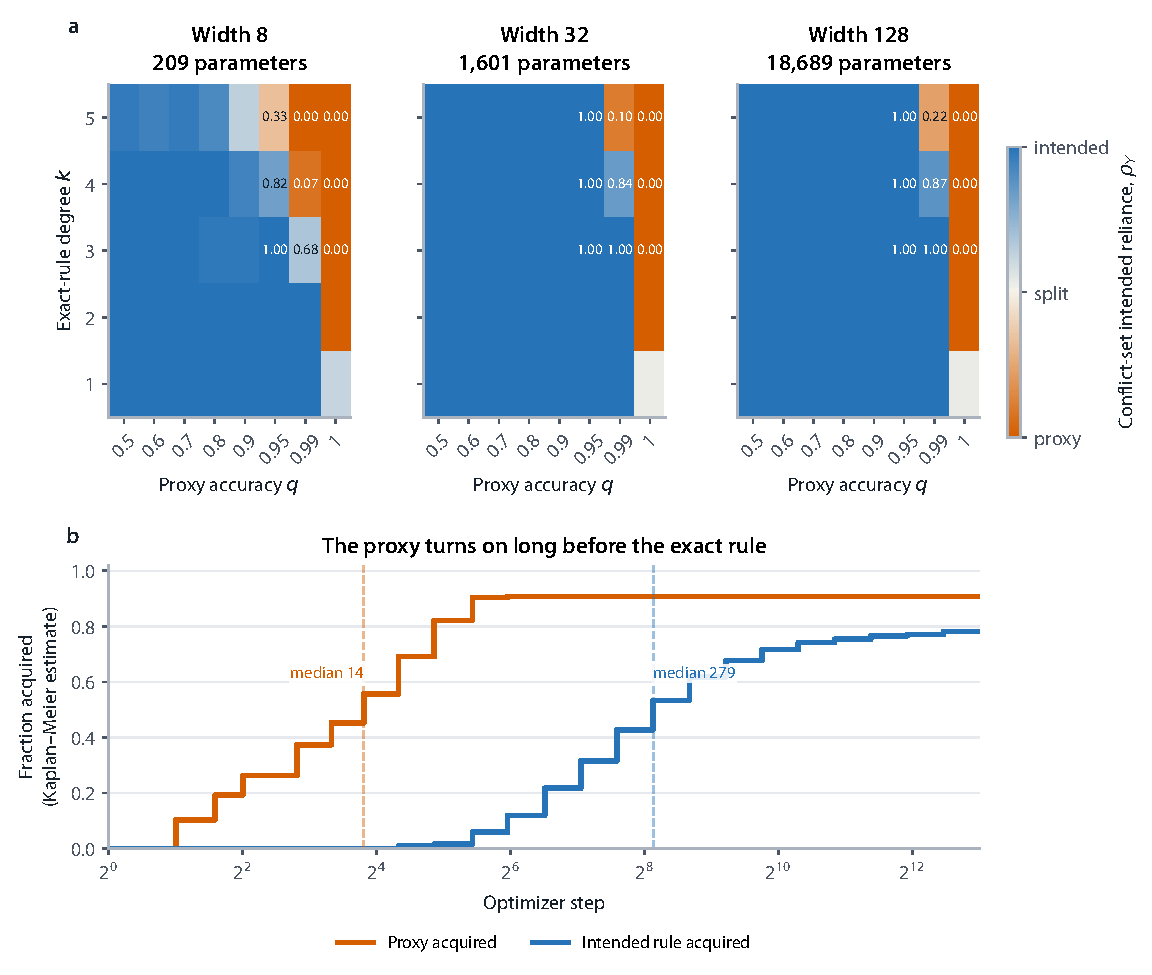
\includegraphics[width=\linewidth]{fig1_phase_and_dynamics.pdf}
  \caption{More reliable proxies and harder exact rules increase proxy control even when in-distribution accuracy is perfect (a). During training, the proxy is typically acquired well before the exact rule (b). Curves in (b) pool the experimental conditions descriptively; the acquisition-order analysis resamples independent training seeds.}
  \label{fig:phase-short}
\end{figure}

We also expected reward to plateau well before the rule controlling behavior stabilized, but this happened in only 13.2\% of identifiable runs; the controlling rule stabilized first in 606 runs, and the logged events tied in 1,372. In this supervised task, learning the exact rule removes a visible residual error, so reward and rule control usually change together at the available checkpoint resolution. The cross-sectional ambiguity of perfect performance therefore does \emph{not} justify the stronger claim that reward generally stabilizes long before the controlling rule.

\begin{takeaway}
In-distribution reward estimates how often candidate rules agree with the labels, not which rule will control behavior where they disagree. Training traces add useful information, but the cheap rule's early lead is not by itself permanent.
\end{takeaway}

\section*{Finding 2: Distinguishing counterexamples matter more than raw data volume}

Repeatedly showing one shortcut failure increases its weight in the loss, but it need not add a new constraint. A flexible model can memorize that exception and keep using the proxy everywhere else. Counterexamples distributed across different contexts are harder to explain as a small patch. With several shortcuts, an example where both fail can also eliminate more candidate explanations than two isolated failures that each leave one shortcut correct.

For alignment data, this means examining the pattern of disagreements, not only the number of labeled examples or proxy errors. We need to know which competing rules each example distinguishes, how varied the disagreement contexts are, and whether the observed combinations of failures still permit a simple rule that switches between shortcuts.

In a diversity experiment planned before full execution, we held training-set size and the total number of proxy conflicts fixed while varying the fraction of distinct conflict contexts. Across 1,500 runs, fully diverse counterexamples raised intended reliance by .299 relative to concentrated repetitions. Every estimable stratum with a fixed conflict count and rule degree showed the same direction. As a descriptive summary, the first tested number of distinct conflicts at which mean reliance reached .9 increased with the difficulty of the intended computation: 32 for the easiest rule, 128 for degrees two and three, and 512 for degrees four and five. These values are crossings on a coarse tested grid, not continuous estimates of sample complexity.

The gap between repeated and novel counterexamples was clearest in the most concentrated condition. Its dataset contained 2,048 presentations of conflicts but only 41 distinct conflict contexts. A five-bit model fit 99.92\% of those repeated conflicts, yet followed the intended rule on only .98\% of unseen conflicts. Flipping the proxy changed 98.39\% of its unseen decisions. The model had learned exceptions to a general proxy rule rather than a general account of why the proxy could fail. \fig{fig:evidence-short} compares conflict count with diversity and shows this gap between repeated and unseen cases directly.

\begin{figure}[!t]
  \centering
  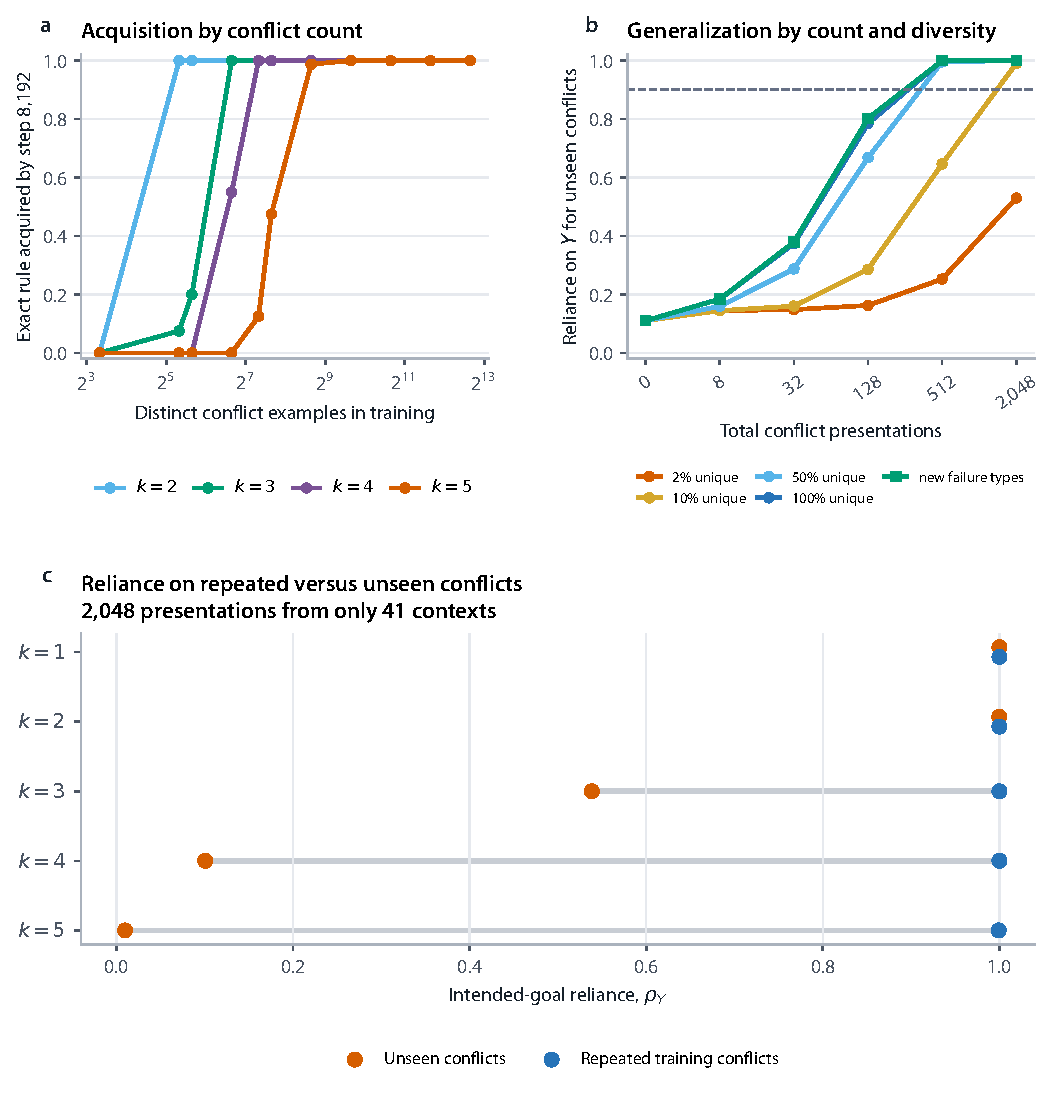
\includegraphics[width=\linewidth]{fig2_counterevidence.pdf}
  \caption{Panels (a--b) show how acquisition of the exact rule changes with the number and variety of conflicts. In panel (c), high-capacity models fit repeated training conflicts nearly perfectly but still follow the proxy on novel conflicts.}
  \label{fig:evidence-short}
\end{figure}

We found a similar pattern with three competing goals. In a factorial experiment planned in advance, reducing the total number of examples on which either proxy failed, while increasing the fraction on which both proxies failed together, shifted causal control toward the intended rule. This average benefit disappeared when the intended parity had degree five: the intended rule accounted for .203 of the normalized feature-flip influence under independent errors and .200 under nested errors. Thus even a highly diagnostic example helps only if the model can learn the intended computation from it. A later follow-up, designed after we had inspected the earlier results, examined a recurring rule: ``use $Y$ when the proxies agree, otherwise use $Q$.'' This rule was almost perfect on every combination of candidate values represented in training, but failed on one combination that the nested-error design excluded. Adding only a few repeatedly sampled rows from that missing combination often destabilized the rule. The effect was not monotonic for every seed or at every dose, so the experiment does not establish a universal sample threshold. Instead, it suggests that missing combinations in the training data can preserve rules that switch among shortcuts.

If this pattern extends to larger systems, ten thousand preference examples that repeat the same kind of evaluator disagreement could reveal less about the learned rule than a smaller set deliberately spanning different reward-model shortcuts. If two plausible objectives almost never fail together in post-training data, a policy can remain compatible with a rule that switches between them. Dataset audits should therefore describe which plausible objectives disagree on which examples, rather than reporting only volume, reward margin, or aggregate error rate.

\begin{takeaway}
When trying to identify the learned goal, we should ask which competing explanations the data rule out. Varied disagreements, examples where several shortcuts fail together, and coverage of missing combinations can matter more than repeated evidence that teaches the same exception.
\end{takeaway}

\section*{Finding 3: An intended rule can be decodable without controlling behavior}

There are at least two thresholds for a candidate goal: the capacity needed to learn or linearly recover it when it is the only target, and the capacity needed for it to win when an easier predictor already explains most of the reward. The second threshold can be higher because little gradient remains to build the harder computation after the proxy has reduced the loss.

For the calibration study, planned before the full runs, we trained separate proxy-only, exact-only, and competition models with matched interfaces. When only a randomly chosen subset of parameters could be updated, the standalone exact decoder met its accuracy criterion at 64 trainable scalars for three-bit parity, but the exact rule did not reliably control the competition model until 1,024 scalars could be updated. At the intermediate budget, decoder accuracy was perfect while intended reliance was .001. Similar gaps appeared for degrees four and five. An exploratory, unadjusted comparison within this architecture grid also found that models matched in parameter count and standalone decoder success could choose different rules in competition. \fig{fig:decode-short} shows the gap between learning a rule on its own and using it when a proxy is also available.

\begin{figure}[!t]
  \centering
  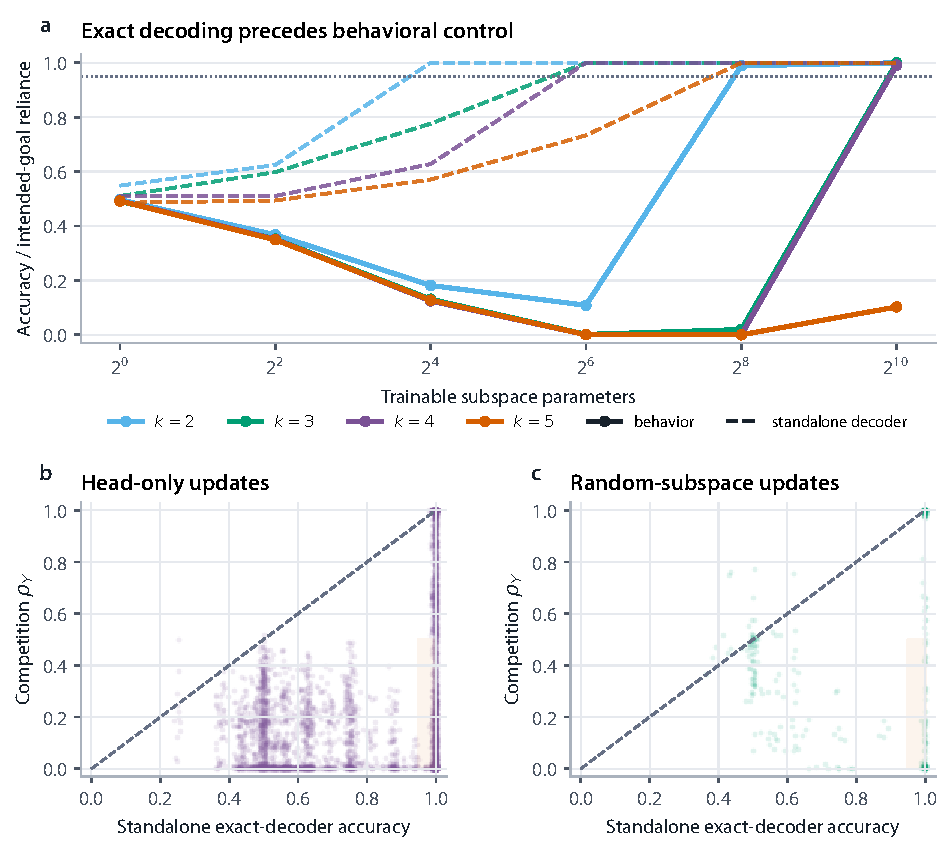
\includegraphics[width=\linewidth]{fig3_decoding_vs_control.pdf}
  \caption{Separate exact-only models can decode the intended rule nearly perfectly even when matched competition models remain proxy-controlled, especially when few parameters can change. The orange region marks high decoder accuracy with low intended-rule reliance.}
  \label{fig:decode-short}
\end{figure}

The distinction between availability and control mirrors a familiar warning from interpretability research: a probe can reveal information in a representation without showing that the model uses it \citep{ravichander2021probing}. Removing or changing that information is needed to connect it to behavior \citep{elazar2021amnesic,vig2020causal}. In \Forkworld{}, the standalone decoder shows that the architecture can learn the intended computation, while disagreement tests and input-channel flips show whether it controls the choice.

The comparison among exact rules also showed that no single numerical measure of ``goal simplicity'' explained the outcomes. In this experiment, planned before full execution, we replaced parity with majority, conjunction, and a multiplexer while keeping the input interface and training exposure fixed. All four exact rules decoded nearly perfectly in isolation. Against a 99\%-accurate direct proxy, mean intended reliance was .100 for parity, .885 for the multiplexer, .985 for conjunction, and 1.000 for majority. This ordering was correlated with how informative the best individual input was: parity offers no useful single-input clue, whereas the other functions provide partial information before the full rule has been assembled. That interpretation is consistent with work showing that Boolean functions and high-degree parities differ in how gradient-based optimization learns them, not only in their input count \citep{malach2019boolean,abbe2025parities}. However, the effects of depth and width were not monotonic, so even the strength of a partial clue is not a complete measure of difficulty.

In a safety audit, this distinction should shape how we interpret internal measurements. Finding a representation of honesty, instruction intent, or a reward-relevant concept would be encouraging evidence that the model can represent that information. It would not establish that the representation governs generation when an easier reward-correlated heuristic points elsewhere. Conversely, a failed linear probe would not establish that the information is absent. A credible claim about behavioral control needs interventions connected to behavior, ideally on inputs where the candidate objectives disagree.

\begin{takeaway}
Success in a separate calibration model shows only that the architecture can learn a rule, not that a competing policy uses it. Even when a probe decodes a rule from the competing model, causal tests are needed to show that the rule controls behavior.
\end{takeaway}

\section*{Finding 4: Training method and history affect which rule wins}

Increasing capability did not always move the model directly from random behavior to the intended goal. In two capacity sweeps planned before full execution, allowing only a small number of parameters to change first made the easy proxy more reliable and therefore made behavior on conflict examples worse. Only after a larger threshold did supervised training replace the proxy with parity. Over this limited range, the result resembles inverse scaling: better in-distribution performance initially meant more consistent pursuit of the wrong rule. This does not imply that capacity is harmful in general. It shows instead that useful computations can become available in an unfavorable order.

To test whether the training algorithm affected which rule won, we compared clean SFT, trajectory SFT, on-policy imitation, and actor--critic RL in an experiment planned before the full runs. All four conditions used the same actor, the same number of presented training examples, and the same core task. Here ``RL'' means that the binary goal selector was trained from terminal success in a simulator with irrelevant intermediate choices; it does not mean that a navigation policy learned to move through the grid. The actor was a 5,897-parameter, two-hidden-layer ReLU network. The actor--critic condition used a separate 35,457-parameter critic, which was never counted toward the limit on trainable actor parameters. At a limit of 1,024 trainable scalar parameters, both SFT variants reached complete intended control and on-policy imitation nearly did, while RL remained completely proxy-controlled. RL did not reliably escape even when all actor weights could be trained. \fig{fig:algorithms-short} shows how the methods diverged as the number of trainable parameters grew. Within this construction, the result is a counterexample to the idea that RL generically avoids proxy lock-in; it is not evidence that SFT is generally safer. It is also relevant to proposals that reward feedback can filter reward-irrelevant variation more efficiently than demonstrations \citep{morris2026reason}.

\begin{figure}[!t]
  \centering
  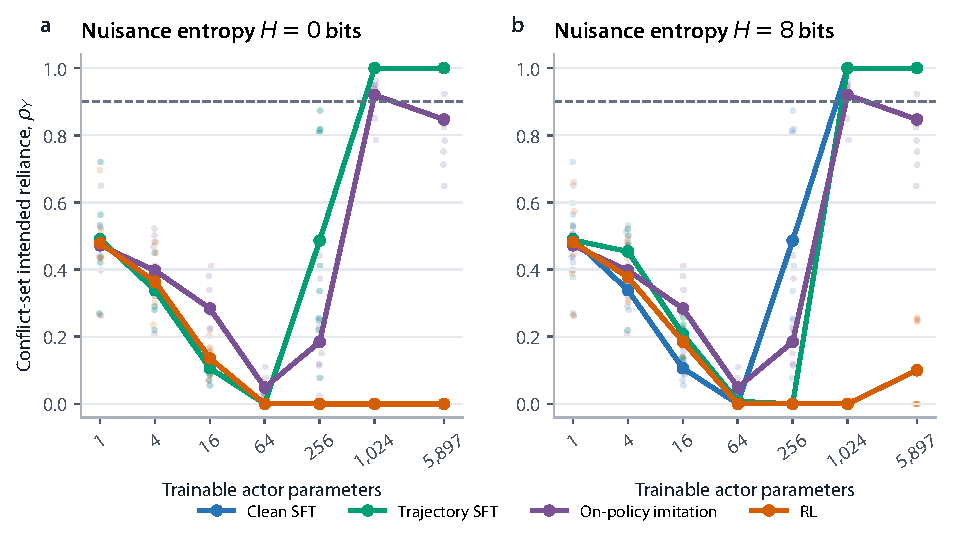
\includegraphics[width=\linewidth]{fig4_update_capacity.pdf}
  \caption{As the number of trainable parameters grows, SFT first learns the proxy and then replaces it with the exact rule. RL does not make the second transition on the tested grid. Points are seeds and lines are means.}
  \label{fig:algorithms-short}
\end{figure}

Several features limit how far this comparison can be taken. The labels for irrelevant intermediate choices were random bits rather than learnable language structure, and RL was not separately tuned at every limit on trainable parameters. Entropy regularization moved a narrow boundary but did not rescue the high-accuracy proxy conditions. Our plan required an improvement of at least .20 before running an additional test of the proposed mechanism; the largest estimate in the expected direction was .125, so we did not run it. The narrower conclusion is that the learning algorithm changed which rule won, and reward-based training provided no automatic protection against this shortcut.

A separate noise study, planned before full execution, produced the opposite of our prediction about averaging over samples. Fresh, zero-mean corruption of the observed proxy did not approach the clean behavioral baseline as the dataset grew. Instead, it weakened the easy route and often redirected learning toward the exact rule. Under the fixed-eight-epoch protocol, larger datasets also meant more updates, so the gap from the clean baseline could grow. Noise tied to a particular state preserved more proxy control than noise sampled afresh, while perturbing labels or rewards produced different effects over training. Calling the noise zero-mean describes the average perturbation; it does not determine the solution selected by a nonlinear optimizer whose trajectory depends on earlier updates.

A later study of training order, designed after we inspected earlier results, showed how prior updates can affect the final rule. Each of six schedules received the same three blocks---one favoring a direct rule, one a two-bit parity rule, and one a three-bit parity rule---in a different order. Afterward, every schedule had seen exactly the same labeled examples, and every named rule was equally accurate on the combined dataset. Nevertheless, the rule favored by the last block controlled all 120 policies. We then trained each model on examples where all three rules agreed. After 256 additional updates, the last rule still controlled 119 of 120 models. \fig{fig:order-short} shows the six orders and the persistence of the last rule during this additional training.

\begin{figure}[!t]
  \centering
  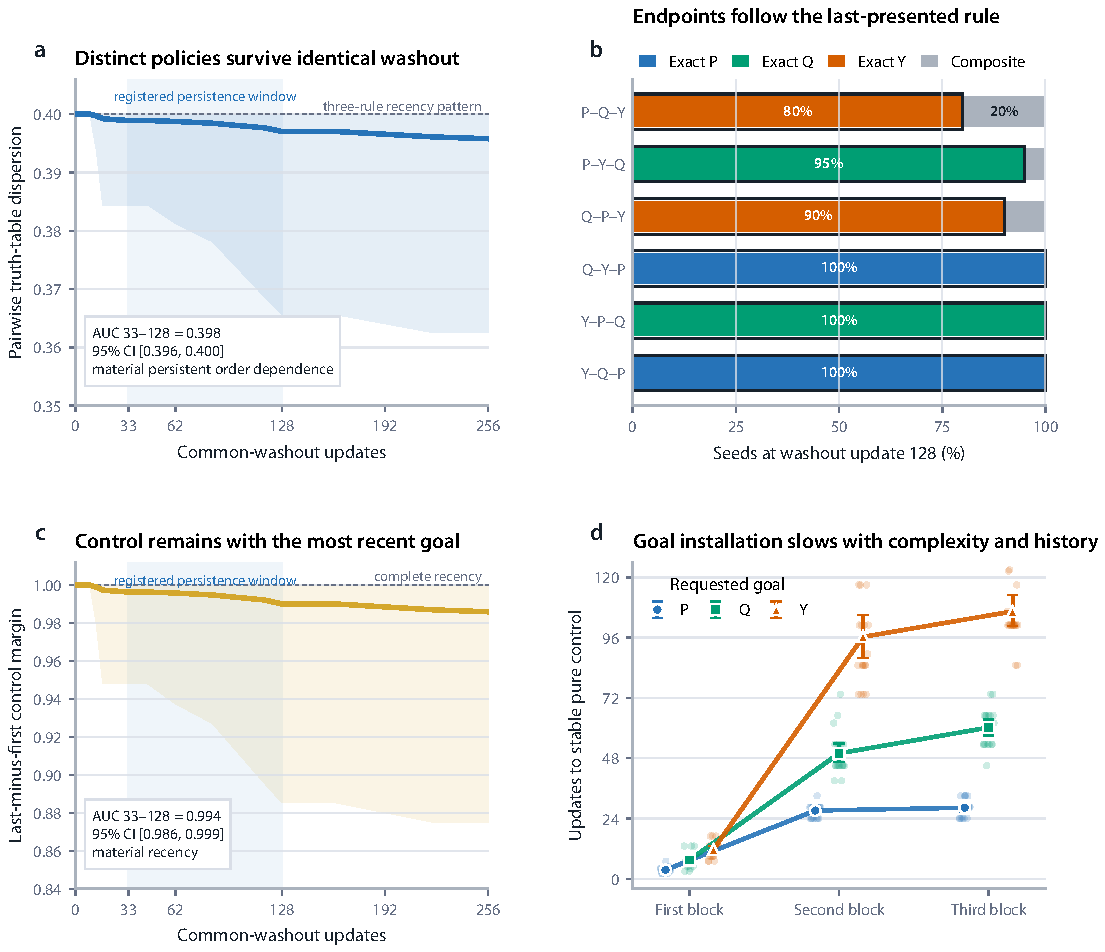
\includegraphics[width=\linewidth]{fig20_identical_evidence_order.pdf}
  \caption{All six schedules receive the same collection of training examples, but the rule favored by the last block remains dominant during a common phase in which all rules agree (a--c). Harder rules and later blocks take longer to establish stable control (d). This follow-up was designed after earlier results had been inspected.}
  \label{fig:order-short}
\end{figure}

Because the combined training objective deliberately assigned equal scores to the rules on the cases where they disagreed, the final data did not identify a unique winner. Reordering whole blocks also changed when their characteristic input patterns appeared. The result therefore demonstrates dependence on training history in this construction; it does not imply that the most recent labels always win. Even so, the unordered collection of training examples was insufficient to predict which rule controlled behavior. The order of the examples, the sequence of optimizer updates, and which rule was already dominant all affected the final outcome.

For LLM post-training, the corresponding research hypothesis is that curricula may install different reward-correlated rules even when aggregate datasets match. Pretraining history, the order of preference data, and late-stage fine-tuning could affect which available rule comes to control behavior. The toy result does not establish that this occurs in frontier models; it identifies order and optimizer history as variables that an alignment evaluation should hold fixed or deliberately vary.

\begin{takeaway}
Goal learning depends on competition during optimization, not only on a static ranking of the candidate labels. Capacity, algorithm, perturbation structure, curriculum order, and weights learned in earlier phases can change the winner even when final performance and the complete collection of training examples look the same.
\end{takeaway}

\section*{Finding 5: Behavior can switch among rules across contexts}

With two candidate goals, a single conflict score encourages us to label the policy ``proxy'' or ``intended.'' Those labels become inadequate once several candidates are available. A model can follow different rules in different parts of the input space, use a context cue to choose among them, or move through several rules over the course of training. Earlier exposure to a rule may still affect later behavior if the dominant rule stops working.

In the context experiment, planned before the full runs, we trained a model on two simple rules, $P_0$ and $P_1$, and supplied a cue $C$ indicating which one would be rewarded. Learning either rule alone required far fewer trainable parameters than switching reliably between them. With restricted updates, both single-rule controls were almost perfect at 64 trainable scalars, while the model chose the context-appropriate rule only .127 of the time; perfect switching appeared at 1,024. At high capacity, fixing $C=0$ made only $P_0$ causally affect behavior, and fixing $C=1$ reversed the responses to feature flips. Forcing the cue to disagree with the actual environment reduced accuracy to chance. \fig{fig:context-short} shows both the capacity needed for switching and the intervention on the cue. The model had learned a manipulable way to select a rule rather than one rule that applied globally, analogous at the input--output level to a learned gate over experts \citep{makkuva2020gated}.

\begin{figure}[H]
  \centering
  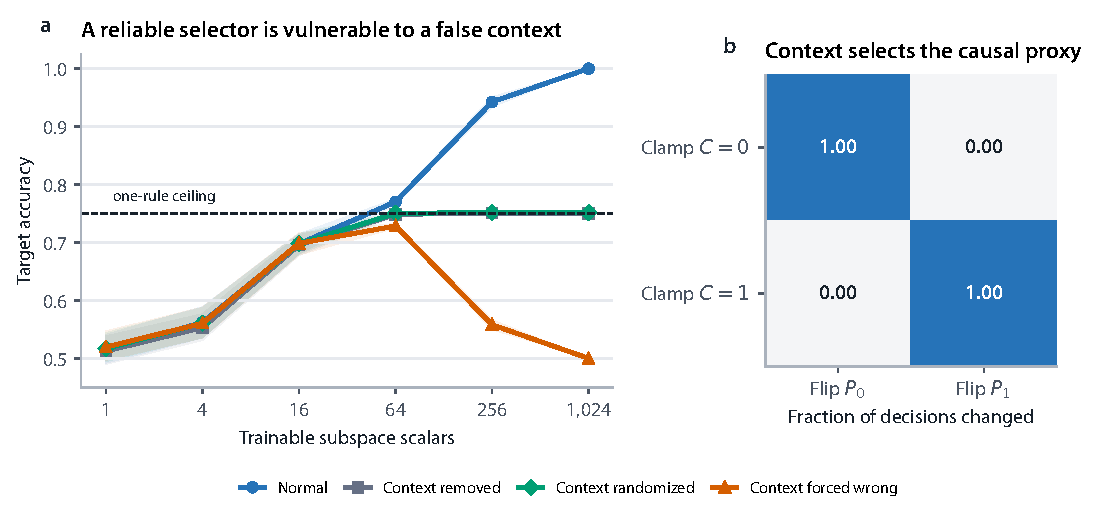
\includegraphics[width=\linewidth]{fig9_context_control.pdf}
  \caption{As switching becomes reliable, setting the context cue incorrectly becomes more damaging (a). At maximum capacity, only the rule selected by the fixed cue causally changes the decision (b).}
  \label{fig:context-short}
\end{figure}

In the three-goal grid, also planned in advance, all three candidate rules decoded perfectly when trained alone. However, only 607 of 960 policies matched the conservative behavioral pattern expected if exactly one named rule controlled every input. In a later check designed after seeing these results, only 102 of the remaining 353 policies behaved like a fixed weighted average of the three named rules. Another follow-up found a recurring alternative: a rule that performed perfectly on the combinations seen during training but failed badly on one missing combination. A policy that did not consistently follow one candidate was therefore not necessarily averaging smoothly among them. It could instead switch according to context, memorize local exceptions, or follow a rule the analyst had not considered.

Later follow-ups tracked how control moved among several rules during training. All 240 models first followed the direct proxy. Many then switched to a second proxy encoded across two input bits before eventually reaching the exact rule. When we made the current winner uninformative, models whose proxies had failed independently switched to the encoded proxy sooner than models with nested proxy failures. The encoded proxy could also be decoded more selectively in the independent-error condition, although the conditions differed in how errors overlapped and in the gradients accumulated during training. Retaining or resetting the optimizer state made a negligibly small difference, which weighs against Adam's stored momentum as the explanation. In this proxy-removal experiment, every model eventually converged to the exact rule. Changing only the two relevant first-layer input columns delayed or accelerated the encoded proxy's takeover as predicted, while equally sized edits to unused columns had practically negligible effects. The weight edits show that first-layer weights connected to a currently inactive rule affected how quickly it later took control. They do not identify a complete circuit, show that the decoded representation causes the effect, or establish that the intermediate rule is a stored utility function.

The timing results did not support a stronger account in which internal decodability always precedes behavioral change. In the follow-up that presented identical sets of examples in different orders, behavioral control and the feature-flip test changed at the same logged checkpoint. Probe timing varied by layer and rule: sometimes before behavior, sometimes at the same time, and sometimes afterward. The data support repeated replacement of the controlling rule and suggest that earlier training can affect how quickly another rule is used later, but not a universal sequence of ``goal acquisition, probe decodability, then behavioral and causal control.''

These results bear on deceptive or conditional behavior only by analogy. They show behavior consistent with several learned rules and a cue that determines which rule governs a particular input; they do not demonstrate situational awareness, concealment, or deception. For LLMs, the corresponding hypothesis is that evaluations should test whether user identity, system prompts, signs of oversight, task framing, or deployment context change which reward-correlated strategy is active. An audit that averages behavior across all contexts can miss such switching.

\begin{takeaway}
In these experiments, behavior changed with context, included exceptions limited to parts of the input space, and sometimes shifted to another rule after the dominant rule failed. Evaluation should therefore test both the cues associated with those changes and the alternative rules that predict behavior, rather than examining only the currently dominant pattern.
\end{takeaway}

\section*{Finding 6: Correct behavior can return while proxy influence remains}

When a proxy stops being rewarded, its old behavior can disappear for several reasons. The model might learn the intended rule, invert the proxy, hide its influence because the feature is absent, or replace it with another shortcut. Accuracy at the end of training alone does not distinguish these mechanisms.

In the persistence study, which was planned before full execution, we first installed proxy control and then either removed the proxy feature, made it independent of the target, reversed its correlation, or introduced a new 99\%-accurate proxy. Negative evidence suppressed behavior consistent with the original proxy faster than simply making the feature unavailable. Under perfect reversal, where $P=-Y$ on every new example, apparently perfect intended behavior was actually complete dependence on $-P$: flipping $P$ flipped every decision, while flipping an exact-code bit changed none. Less extreme reversal included rare rows that distinguished $-P$ from $Y$, and the models eventually transferred control to the exact rule. \fig{fig:unlearning-short} distinguishes suppression of the old behavior, residual dependence on the old feature, and control by the inverse proxy.

When we replaced the old shortcut with a new one, performance on the current distribution recovered before dependence on the old rule disappeared. The model reached nearly perfect accuracy and strong agreement with the replacement proxy after about 18 updates, while behavior consistent with the old proxy took about 59 updates to fall by half. A high-performing model at the end of training can therefore retain some dependence on an old shortcut while also learning a new one.

\begin{figure}[H]
  \centering
  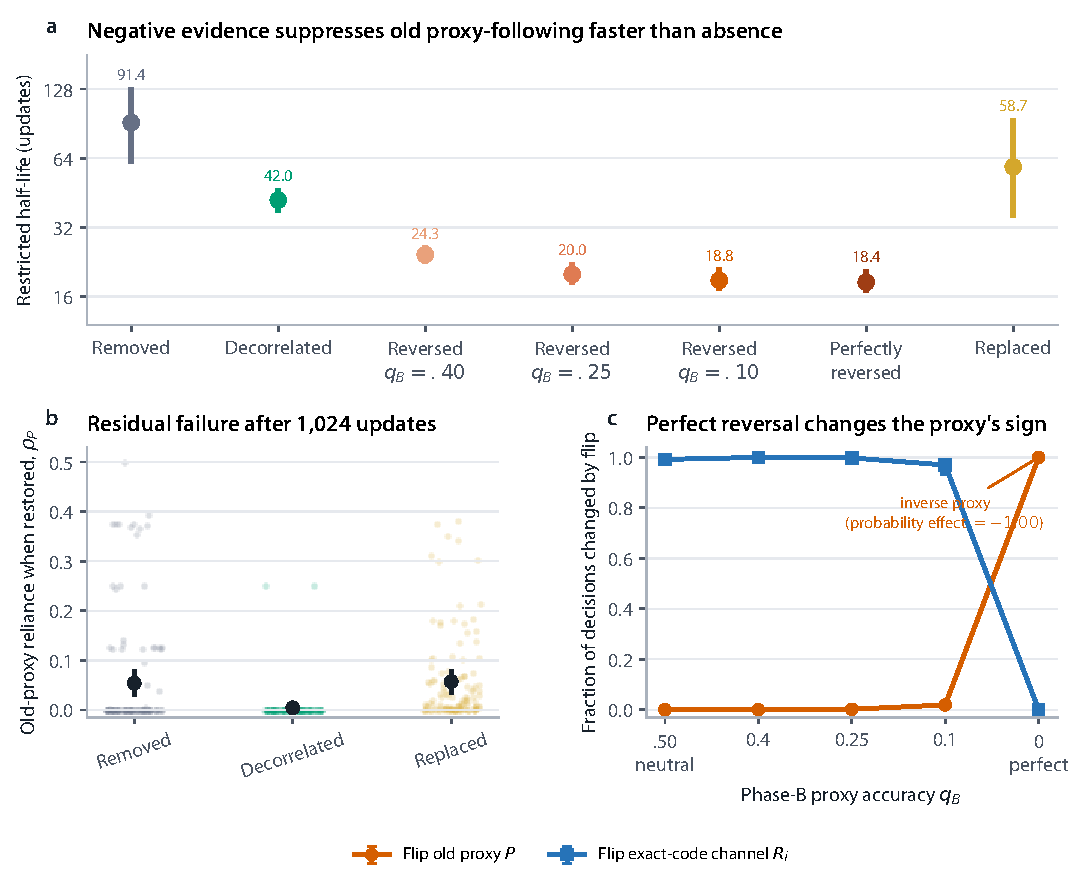
\includegraphics[width=\linewidth]{fig6_unlearning.pdf}
  \caption{Negative evidence suppresses behavior consistent with the old proxy faster than removing the feature (a). Restoring the input reveals residual dependence (b), and perfect reversal installs the inverse proxy rather than the exact rule (c).}
  \label{fig:unlearning-short}
\end{figure}

In the rebound experiment, also planned in advance, we compared models with three histories: prior training on the old goal, an equal amount of training on random labels, and no relevant prior training. After all groups were brought to similar visible behavior, ambiguous later training produced nearly equal final reliance on the old goal within each matched perturbation condition. The difference in rebound between old-goal and random-label histories stayed within the five-percentage-point range we had defined as practically negligible. Most of the large raw rebound was therefore renewed learning of an easy proxy, rather than evidence that the old objective had remained dormant. This matched comparison is especially relevant to reports of post-alignment ``elasticity,'' in which models move back toward pretraining behavior \citep{ji2025alignment}.

Although prior old-goal training did not explain the final rebound, it did increase the amount of evidence required for realignment. Among the matched conditions that qualified for this analysis, models previously trained on the old goal needed 1,046 additional intended-goal examples after the shortest old history, and 15,677 after the longest, to enter the same behavior range as models that had instead trained on random labels. Qualification for the analysis depended strongly on model width, and the estimate at the largest data volume used only eight seeds, so these numbers do not establish a clean scaling law. They do show that training history can affect how quickly behavior changes without uniquely explaining the model's eventual behavior.

Claims about objective erasure, sleeper behavior, or post-fine-tuning reversion should therefore be supported by causal interventions and matched controls. If a model returns to a shortcut after ambiguous data, it should be compared with both a model trained from scratch and one given the same amount of earlier training on an irrelevant task. If behavior becomes correct after reversal, interventions should test the original feature and its inverse. If a probe remains strong, the audit should test whether intervening on the corresponding representation changes behavior. None of these tests identifies a unique motivation by itself, but together they rule out several simpler explanations.

\begin{takeaway}
In these experiments, correct behavior sometimes returned while dependence changed sign or moved to another shortcut. Rebound alone did not establish continued causal influence from the earlier rule, because matched controls often reproduced it.
\end{takeaway}

\section*{Synthesis: five ingredients for predicting behavioral control}

The experiments do not support ``the simplest goal wins'' as a sufficient theory. The results are better organized around five more specific considerations.

\begin{enumerate}[leftmargin=*,itemsep=0.45em]
  \item \textbf{Which examples distinguish the rules.} When candidate goals agree on the training data, the data cannot tell us which one the model follows. Varied disagreements, examples where several proxies fail together, and coverage of all relevant combinations determine which alternatives are actually ruled out.
  \item \textbf{How easily this model can learn each rule.} Useful partial clues, network architecture, and which parameters can be updated all affect how readily a model can build a rule. The number of input channels and accuracy of a standalone decoder do not fully describe how difficult the rule is for a particular model to learn.
  \item \textbf{Competition during training.} A cheap predictor can absorb most of the early gradient and leave little signal for harder alternatives. Capacity, learning algorithm, entropy, and noise can change the sequence in which rules are learned and which one controls behavior.
  \item \textbf{Combining and switching between rules.} A policy can use context to choose a rule, memorize exceptions for parts of the input space, or hand control from one rule to another during training. In some conditions, it was inaccurate to describe every policy as either one rule used everywhere or a fixed weighted average.
  \item \textbf{Training history.} What the model learned earlier, together with the order of later examples, affects which alternative takes control. The same complete collection of examples can produce different behavior when those examples do not distinguish among the candidate rules.
\end{enumerate}

These five considerations are a checklist rather than a fitted theory. Several experimental manipulations changed more than one of them, and all were tested in a small synthetic setting. The checklist is useful because it replaces a vague appeal to ``simplicity'' with properties that can be measured, manipulated, and tested.

\section*{Implications for alignment evaluations}

Because these experiments use small synthetic models, their most direct implications concern how to design evaluations rather than what to conclude about the internals of frontier models.

\begin{enumerate}[leftmargin=*,itemsep=0.5em]
  \item \textbf{Construct explicit disagreement sets.} List several plausible rules that could explain reward---for example instruction following, evaluator approval, stylistic conformity, sycophancy, or a reward-model artifact---and create cases where their recommended outputs diverge. Ordinary in-distribution validation cannot identify control when the candidates agree.
  \item \textbf{Check which rules the post-training examples distinguish.} Report distinct failure contexts, examples where several proxies fail together, and combinations that are absent, rather than only dataset size. Counterfactual preference examples are useful when they isolate which candidate explanation is contradicted \citep{kaushik2020difference}.
  \item \textbf{Separate availability from use.} Use probes to identify information that may be available to the model, then pair them with behavioral disagreements, causal feature or representation interventions, and negative controls before claiming that the information controls output.
  \item \textbf{Evaluate trajectories and curricula.} Save checkpoints before, during, and after alignment; permute evidence order where possible; and vary optimization algorithms, entropy or exploration settings, and model capacity. A final reward number can hide an early proxy regime, a later handoff, or persistent order dependence.
  \item \textbf{Test whether context changes the active rule.} Intervene on oversight cues, system prompts, user identities, task frames, and other contextual variables that may switch the model between strategies. Use several sets of disagreement examples so that a rule that changes with context is not incorrectly described as one globally dominant goal.
  \item \textbf{Use matched histories for claims about unlearning.} Compare old-history models with scratch and compute-matched controls under identical later data. Test inverse shortcuts and replacement proxies. Report both final behavior and the amount of evidence required to reach it.
\end{enumerate}

When applied to RLHF or other LLM post-training, these recommendations should be treated as research hypotheses. Reward-correlated linguistic shortcuts may compete with intended behavior; the pattern and order of preference examples may determine which rule takes control; and deployment cues may activate a strategy used only in some contexts. \Forkworld{} does not show that any particular frontier model has these properties. It provides a small setting in which apparently similar claims can be separated experimentally, along with a basis for designing stronger tests.

\section*{Limitations and next steps}

\Forkworld{} uses small ReLU MLPs, binary actions, synthetic Boolean rules, and mostly one-step choices. Parity is a clean way to remove lower-order clues, not a claim that real goals have polynomial degree. Ten optimizer seeds quantify variation inside the tested conditions, not uncertainty over model families, objectives, or deployment environments. The navigation controller is frozen and works mainly on maps like those used to train it; the repeated-fork extension adds walls and multiple decisions but not learned planning, memory, or recovery. Reliance and feature flips identify causal control only among the candidate rules and interventions we constructed.

The way the studies were planned also limits the conclusions. Thirteen experiment families were specified in advance within the project, but they were not publicly preregistered. The six follow-ups were chosen to explain patterns in earlier results, and confidence intervals do not remove the bias introduced by that choice. In particular, the effects of training order, the sequence of control changes among several goals, the addition of previously missing input combinations, the removal of a dominant rule, and edits to features used by a backup rule should all be replicated in new model families before being treated as general mechanisms.

The next step is to scale the framework to LLMs using naturalistic competing objectives, independent sets of disagreement examples, checkpoints throughout training, and matched interventions on candidate representations. Richer game environments should jointly train perception, memory, navigation, and goal selection under partial observability, multiple forks, changes of context, and opportunities to recover from mistakes. These settings would make causal attribution harder, but would test whether the five considerations above still predict which rule controls extended reasoning and action.

\clearpage
\appendix
\begin{center}
  {\LARGE\bfseries Appendix}
\end{center}
\vspace{1em}
\section{Environment and agent specification}
\label{sec:environment-specification}

\subsection{Trainable components and task structure}

The experiments primarily train a \emph{goal selector}, rather than an end-to-end grid-navigation policy. The selector receives signals for the candidate goals together with task-irrelevant input coordinates, and produces one binary logit for choosing the left or right target. Supervised runs train this logit against the intended binary action. In the RL runs, the logit parameterizes a Bernoulli policy that is trained from the reward for the resulting outcome. The selector never receives pixels or a grid observation in the primary factorial analyses.

The project uses four environment levels, summarized below. Coordinates are zero-indexed $(\text{row},\text{column})$. At the first three levels the selector makes at most one target choice. In the fixed-fork and obstacle-grid variants, that choice is then passed as an explicit one-hot goal ID to a separately pretrained and frozen navigator. RouteWorld is different: the same selector supplies one branch bit for each reward-relevant fork, while a scripted controller executes every forced corridor move.

\begin{table}[!htbp]
\centering
\small
\begin{tabularx}{\linewidth}{@{}p{0.17\linewidth}p{0.29\linewidth}X@{}}
\toprule
Level & Environment and horizon & Learned choice and movement \\
\midrule
One-step choice & No spatial grid; horizon one. & The selector chooses $-1$ or $+1$. Reward is one iff that choice equals the intended label $Y$. This is the level used for the main factorial estimates and causal channel interventions. \\
Fixed fork & A $7\times7$ wall grid with 12 walkable cells. Start $(6,3)$; fork $(3,3)$; targets $(1,1)$ and $(1,5)$; horizon seven. & The selector chooses one target before rollout. Both shortest routes have seven primitive moves. On an expert route, the sole goal-dependent navigation decision is LEFT versus RIGHT at the fork; all other progress follows the corridor. A frozen navigator executes the route. \\
Obstacle grid & A $9\times9$ grid with requested obstacle probability $.22$ and horizon $2HW=162$. The start is sampled in rows 6--8; the left target in columns 0--3 and the right target in columns 5--8; each is at least four Manhattan steps from the start. Disconnected paths are carved open. & The selector again chooses one target. A frozen navigator handles genuine obstacle-dependent movement. Scientific summaries use the 32 maps on which that navigator was pretrained; unseen layouts are reported separately as a capability control. \\
RouteWorld & A perfect binary tree embedded in walls. Depths $D=1,2,4$ give grids $4\times5$, $7\times9$, and $13\times33$, with route lengths $4,9,27$ and $2^D$ visually identical terminal leaves. & Before rollout, the selector computes $D$ left/right choices from $D$ stage-indexed input rows. It sees padded route signals and a one-hot stage address, but no target marker, tree node, or history state. A scripted controller then executes the route. \\
\bottomrule
\end{tabularx}
\caption{The four task levels. The fixed fork is a small T-shaped corridor with one meaningful branch, whereas the obstacle environment is a conventional navigation grid with a single goal choice made upstream. RouteWorld adds repeated goal-relevant choices without learning corridor navigation.}
\label{tab:environment-levels}
\end{table}

RouteWorld does not train a policy from the physical maze observation. This observation has three flattened channels---agent position, walls, and generic terminal leaves---and does not identify the rewarded leaf or its route. The selector instead receives a fixed 44-dimensional vector: four padded proxy bits and four presence masks, sixteen padded exact-code bits and sixteen corresponding masks, and a four-way one-hot stage address. The complete route signals are repeated at each stage; only the stage address changes. The implementation evaluates all $D$ stage rows, converts their logits into a complete sequence of branch choices, and gives that sequence to the scripted corridor controller for physical verification. RouteWorld therefore measures repeated local goal selection and the accumulation of errors across forks. It does not test learned perception, online planning, a policy with memory, dependence on earlier branch outcomes, or recovery after a wrong turn.

The fixed fork's walkable layout is
\begin{center}
\begin{minipage}{0.28\linewidth}
\begin{verbatim}
#######
#L###R#
#.###.#
#..F..#
###.###
###.###
###S###
\end{verbatim}
\end{minipage}
\end{center}
where \texttt{S} is the start, \texttt{F} is the only goal-dependent fork, \texttt{L/R} are terminal targets, and \texttt{\#} denotes a wall. The two shortest action sequences are \texttt{UUULLUU} and \texttt{UUURRUU}. Reaching either target terminates the episode; physical reward is one only when it is the designated target. Collisions leave the agent in place and still consume a step.

\subsection{Selector architectures and trainable parameters}

The baseline selector input has 15 scalars: the fixed prefix $(P,P_{\mathrm{present}},R_1,\ldots,R_5)$ plus eight task-irrelevant state coordinates. Inactive $R_i$ positions are padded so that changing the parity degree does not change the input width. The default model is a non-residual MLP with two 64-unit ReLU hidden layers, biases, and one binary goal logit, for a total of 5,249 parameters. Individual experiments vary the width, depth, activation function, use of residual connections, or set of trainable parameters, as listed in the protocols below. When an experiment imposes a random-subspace limit $U$, it freezes the base network and trains exactly $U$ scalar coordinates through a fixed random count-sketch projection. The setting marked ``full'' trains every parameter.

The E5 algorithm comparison and the E10/E14 entropy studies use a matched 5,897-parameter actor. Its 17-dimensional input adds one reward-irrelevant context bit and one coordinate that records the binary path produced by the policy's preceding branch choices. It has the same two 64-unit ReLU hidden layers, followed by one goal head and eight binary heads for reward-irrelevant branch choices. All algorithm conditions retain all heads even when a head contributes no loss, keeping the actor architecture and number of trainable parameters fixed.

For actor--critic RL, sigmoid probabilities define the sampled binary actions. In E5, up to eight neutral branch actions are sampled before the final goal action; each neutral branch reconverges and cannot change success. The complete simulator horizon is 17 primitive actions---eight branch choices, eight forced merges, and the terminal goal choice---and the actor never observes a demonstration label for a neutral branch. It receives one terminal outcome, equal to one iff the final selected goal is correct. The policy loss uses the sum of sampled-action log probabilities times a normalized advantage, plus the configured entropy bonus. Evaluation is greedy.

The E5/E10/E14 critic is a separate 17-input scalar network with three width-128 residual GELU hidden transformations and 35,457 parameters. It is fully trained with squared reward-prediction loss and is excluded from every limit on trainable actor parameters. Actor and critic use AdamW. The standard setting uses 2,048 updates, a batch size of 250, a learning rate of $.003$, and zero weight decay, for a total of 512,000 presented contexts. E5 compares training every actor parameter with training exactly $U\in\{1,4,16,64,256,1024\}$ scalar coordinates. The E6 noise experiment uses the same width-64, two-hidden-layer actor design with a 16-dimensional interface and 5,833 parameters, but its fixed critic has width 256, depth three, and 136,193 parameters. E6 follows a fixed eight-epoch dataset schedule, so its update counts depend on dataset size and are specified in its protocol.

\subsection{Frozen navigation policy}

The navigator sees four flattened binary grid channels---agent position, obstacles, left target, and right target---plus a two-entry one-hot selected-goal ID. It is an MLP with two 128-unit ReLU hidden layers and four output logits for UP, RIGHT, DOWN, and LEFT. The fixed-fork instance therefore has 198 inputs and 42,500 parameters; the obstacle-grid instance has 326 inputs and 58,884 parameters. These navigator parameters are not included in any limit on trainable selector or actor parameters. The navigator is trained by supervised imitation of deterministic breadth-first-search shortest-path actions, rather than by RL, with AdamW, batch size 128, learning rate $.003$, zero weight decay, and a maximum of 250 epochs.

The fixed-fork navigator is trained on all 20 reachable goal-conditioned state--action rows and reaches 100\% action accuracy after 67 epochs. The obstacle navigator is trained on 3,908 rows from 32 generated maps and reaches 99.795\% after 29 epochs. Training stops after the requested $.99$ accuracy is sustained for three epochs; both networks are then frozen. For experiment families that enable sequential checks, each selector is evaluated with 128 fixed-fork and 128 obstacle-navigation rollouts. The obstacle-grid evaluation cycles through the 32 maps used for navigator training four times; it does not create 128 new layouts. These rollouts check that the selector's target choice can be passed to a competent controller on familiar maps. They are repeated measurements of the selector, rather than independent training runs. Held-out obstacle maps are reported as a separate capability check because the frozen navigator performs poorly on them.

\section{Shared construction, evaluation, and inference}

The original nine families use seeds
\[
\{11,23,37,41,53,67,71,83,97,101\}.
\]
Unless a family below overrides it, training, validation, and conflict sets contain 10,000, 4,000, and 10,000 rows; batch size is 250; learning rate is .003; AdamW weight decay is zero; and the global gradient norm is clipped at one. Eight task-irrelevant coordinates accompany the proxy and exact-code inputs. Requested proxy accuracies are constructed exactly rather than sampled only in expectation.

The default acquisition event requires a score of at least .9 at two consecutive logged checkpoints. Multi-goal pure control requires both behavioral agreement and directional causal control at least .9, each with a .1 margin over the other named candidates, at two checkpoints. Standalone decoder success usually uses .95 accuracy. These thresholds discretize continuous trajectories and do not establish literal phase transitions.

Causal evaluation changes one candidate channel on matched base inputs. In the parity baseline, flipping $P$ reverses the proxy recommendation, while flipping one active $R_i$ reverses the exact decoded $Y$. Reliance uses hard actions; probability and logit effects are secondary diagnostics. A probe is always interpreted as decodability, never as a goal label or proof of control by itself.

Intervals use 4,000 bootstrap resamples of training seeds at 95\% confidence. Matched conditions are differenced within seed before resampling. When specified by the analysis plan, repeated cells that differ only in task-irrelevant variables are first averaged within seed. The independent unit is always the trained initialization seed, never an evaluation row, episode, checkpoint, schedule, duplicated control, or scripted rollout. Analyses of when an event occurs preserve the checkpoint interval in which it occurs and retain runs that never reach the criterion as right-censored. Restricted means use the fixed experimental horizon. Areas under curves use linear-in-update trapezoids between directly observed checkpoints.

\section{Experiment protocols}

\subsection{E1--E5: learning order, counterexamples, capacity, and algorithms}

\textbf{E1.} A two-hidden-layer ReLU selector trains for 2,048 full-parameter update steps. The experiment crosses eight proxy accuracies $q\in\{.50,.60,.70,.80,.90,.95,.99,1\}$, five parity degrees, five widths $8,16,32,64,128$, and ten seeds. The primary statistic is the within-seed Spearman association of $q$, $k$, or capacity with $\rhoY-\rhoP$. The reported first crossings are limited to the tested grid values and should not be read as continuous sample-complexity estimates.

\textbf{E2.} At $q=.9$, separate proxy-only, exact-only, and competition models train for 4,096 steps with the same input width and parameterization. Full and head-only updates cross degrees 1--5, depths 1, 2, and 4, widths 8--128, ReLU/tanh/GELU activations, and residual connections on/off. A fixed width-128, depth-4 residual ReLU model adds random-subspace budgets $U\in\{1,4,16,64,256,1024\}$. The exact-decoding threshold is .95 final accuracy in eight of ten seeds; competition requires $\rhoY\geq.9$ in eight of ten.

\textbf{E3.} The 8,192-update training-dynamics experiment crosses five proxy accuracies, parity degrees 2--5, datasets of 1,000, 4,000, or 16,000 rows, four widths, and ten seeds, with 25 logarithmically spaced checkpoints. Acquisition and replacement require the relevant criterion to hold at two consecutive checkpoints. A reward plateau is defined as the first four-checkpoint window whose range is at most .005, whose level is close to terminal reward, and whose value exceeds a $q$-dependent floor. The prospectively specified joint prediction required the lower confidence bounds for both the simple-first and plateau-first fractions to exceed .5. The simple-first prediction passed this criterion, whereas the plateau-first prediction did not.

\textbf{E4.} Total $N=10,000$ is fixed while requested conflict counts $0,8,32,128,512,2048$, degrees 1--5, and unique-context fractions 2\%, 10\%, 50\%, and 100\% are crossed. Evaluation IDs are disjoint. The diverse-minus-concentrated contrast matches conflict count, $q$, $k$, and seed. A structured arm trains on two invertible failure transformations and tests two disjoint transformations.

\textbf{E5.} A 5,897-parameter actor with eight auxiliary heads for reward-irrelevant choices is shared by four algorithms. Clean SFT labels only the goal action. Trajectory SFT also applies a negative-log-likelihood loss to active, randomly labeled auxiliary branches. On-policy imitation samples two transitions from the current policy and queries the same minimal action oracle, while actor--critic RL uses terminal success reward. Four auxiliary-branch levels, six random-subspace limits $U\in\{1,4,16,64,256,1024\}$ plus full-parameter training, and ten seeds give 1,120 runs. Every condition receives 2,048 optimizer steps and 512,000 presented training contexts. A fixed width-128, depth-3 critic is excluded from the actor parameter limit. Full-parameter and random-subspace updates are not nested, so first crossings on this grid do not show that adding trainable coordinates causally reduces performance.

\subsection{E6--E9: perturbations, prior training, and context-dependent rules}

\textbf{E6.} This experiment crosses four algorithms; step-resampled, episode-static, state-static, and target-correlated biased perturbations; perturbations to the proxy observation, imitation label, or reward; five scales $0,.25,.5,1,2$; recurrence of $1,4,16,$ or 64 episodes per underlying state; three dataset sizes; and ten seeds:
\[
(4)(4)(3)(5)(4)(3)(10)=28,800.
\]
It fixes $q=.9$, $k=3$, a width-64 two-layer selector, batch size 256, and eight dataset epochs. Dataset sizes 2,560, 10,240, and 40,960 imply 80, 320, and 1,280 updates. Each episode repeats one contextual choice for four rows: step noise redraws per row, episode noise is shared across four rows, and state noise is fixed whenever the goal-relevant variables have the same underlying values. Biased noise adds $bY$, where $b=\min(.25,\sigma)$, while adjusting residual Gaussian variance.

The primary temporal contrast uses 7,680 positive-scale runs in which the proxy observation is perturbed, together with 1,920 matched zero-scale controls. Within every seed and combination of experimental conditions, it defines $g(N)=\rhoY(\sigma>0,N)-\rhoY(\sigma=0,N)$ and fits OLS slopes of $g(N)$ and $-|g(N)|$ against the base-two logarithm of the number of presentations before averaging the planned combinations. The scaling result must replicate separately in clean SFT and RL. Another 9,600 cells are exact negative controls because the perturbed variable does not enter the algorithm's training objective. A separate 100-run terminal-reward experiment fixes RL, reward noise, $N=10,240$, and recurrence 16 to compare step-level and episode-level perturbations when only one reward is emitted per episode. The repeated contextual rows are not sequential-policy rollouts. Increasing recurrence also reduces the diversity of underlying states, so these two factors are not separately identified. Target-correlated noise is a different intervention, rather than another degree of temporal persistence.

\textbf{E7.} Phase A trains the model to rely on the original proxy at $q_A\in\{.9,.99,1\}$ over widths 16--128, requiring reliance of at least .9 at three evaluations within 4,096 updates. Phase B resets the optimizer and runs for 1,024 updates after the original proxy is removed, decorrelated from the target at $q_B=.5$, reversed at $q_B=.4,.25,.1,0$, or replaced by a new .99-accurate proxy. Removal masks both $P$ and its presence bit. To test whether the original proxy still affects behavior, the evaluation restores it on a balanced set of conflicts. The proxy's half-life is operationally defined as the first time reliance falls below half its Phase-A value; one removal run never crosses this threshold and is retained as right-censored at the experimental horizon. The primary 840 runs are supplemented by 1,080 sensitivity runs at weight decay $10^{-5},10^{-4},10^{-3}$.

\textbf{E8.} Models in the old-history condition first receive $N_0\in\{512,2048,8192,32768\}$ examples labeled by the proxy. Compute-matched controls receive the same amount of training with balanced random labels, while no-history models skip this stage. Intended realignment either uses a fixed 8,192 examples or continues until behavior reaches a .90--.93 target band. Four final conditions run for 2,048 optimizer updates: one provides only examples on which the old and intended goals agree, one also removes the intended-goal channels, and two label disagreement cases according to the old goal 55\% or 75\% of the time. Reactivation requires old-goal reliance of at least .9 at two logged checkpoints and retains interval censoring. The complete grid contains 2,880 runs, but only 479 of 720 distinct cells meet the pre-perturbation inclusion criterion before the four final conditions are replicated. History comparisons use the compute-matched random-label control. Because inclusion depends strongly on model width, the results do not by themselves support broad scaling claims.

\textbf{E9.} Two independent rules $P_0,P_1$ and a balanced unobserved environment variable $E$ define the target $Y=P_E$. During training, the observed context satisfies $C=E$ and $C_{\mathrm{present}}=1$. Full-parameter updates cross seven widths, three depths, and ten seeds; a fixed large residual network adds six random-subspace budgets. Every selector is paired with two single-rule calibration models. The planned analysis retains only runs in which both calibration models reach .9; 38 calibration runs fail this requirement. The raw architecture heatmaps intentionally include all runs. To evaluate strict switching, the analysis takes rows on which the two rules disagree and evaluates each row twice, once with the context fixed to each possible value. Context randomization and forced mismatches preserve $E$, $P_0$, $P_1$, and the target while altering only $C$; context removal sets $C=0,C_{\mathrm{present}}=0$.

\subsection{E10--E13: entropy, alternative rules, multiple candidates, and repeated forks}

\textbf{E10.} The E5 actor--critic is trained for 2,048 updates over four proxy accuracies, three parity degrees, six entropy coefficients $0,.003,.01,.03,.1,.3$, and ten seeds, giving 720 runs. REINFORCE and a 1,024-scalar actor subspace add 120 controls for the pre-specified reference setting. Reliable control requires eight of ten seeds above .9. The decision rule specified before the experiment required an improvement of at least .20 with a positive confidence interval before running the planned mechanism panel. The largest estimate with the predicted sign was .125, so that panel was not run. E14 is a separate post-hoc response to a different setting.

\textbf{E11.} Balanced five-bit parity, majority, and conjunction, plus a six-bit multiplexer, share a six-channel padded interface. Four rules, three proxy accuracies, five widths, two depths, and ten seeds give 1,200 runs. Separate proxy, exact-rule, and competition models train for 4,096 updates. Exact-rule calibration runs repeated across $q$ are bit-identical, rather than independent decoder replications. The causal tests change the minimum possible number of input bits needed to flip each rule. Because these Boolean interventions can differ in size, their effects on output probability are not compared directly across rules.

\textbf{E12.} A direct proxy $P$, parity-coded proxy $Q$, and exact parity-coded $Y$ share one selector. The 960-run grid crosses two $q_P$ values, three $q_Q$ values, two $Q$ degrees, two $Y$ degrees, two widths, independent versus maximally nested error patterns, and ten seeds. The error rate of each proxy is fixed exactly. In the independent condition, their overlap is the nearest finite-sample value to the product of the two error rates; in the nested condition, the smaller set of errors lies wholly inside the larger set. Candidate calibration and competition models use matched masked inputs and 2,048 full-parameter update steps. Three 10,000-row evaluation sets make both proxies wrong, only $P$ wrong, or only $Q$ wrong. A model receives a pure-control label only when its closest behavioral pattern agrees with the candidate that has the largest causal influence, its error on the relevant evaluation set is at most .10, and directly flipping that candidate changes the action on at least half of cases. ``Mixture or unresolved'' is a conservative negative classification, not evidence of literal internal mixing. A post-hoc model check also attempted to reconstruct the output as a fixed additive combination of candidate rules, but this check was not part of the prospective decision rule.

\textbf{E13.} RouteWorld embeds an equal-depth binary decision tree in walls. A scripted controller executes the corridors, while the selector sees every route channel and a one-hot stage address. Depths 1, 2, and 4, three proxy accuracies, two parity degrees, two widths, two training-allocation regimes, and ten seeds give 720 runs, each with 4,000 exactly balanced route episodes. Fixed-total models receive 1,024 updates; per-fork-matched models receive $1,024D$. Evaluation includes in-distribution routes, routes on which all stages place the proxy and exact rule in conflict, and routes with one conflict stage at a time. The pre-specified approximation to whole-route success raises the pooled branch accuracy to the power $D$; a separate calculation that multiplies the measured accuracy at each stage is exploratory. The two depth-one training regimes are duplicate controls. Physical rollouts are repeated measurements, so this experiment tests repeated local selection rather than learned planning or memory.

\section{Follow-up protocols}

\textbf{E14: timing of entropy regularization.} After inspecting E10, the analysis selected the responsive $q=.75,k=4$ setting and the pre-specified $q=.9,k=3$ reference setting for six schedules: no entropy, continuous entropy coefficient $.3$, early-only entropy, delayed-only entropy, delayed entropy with an actor-optimizer reset, and delayed entropy with a critic and critic-optimizer reset. The schedule changes at update 64 of 2,048. All 120 runs use the E5 actor--critic and the ten original seeds. The primary endpoint is final intended-rule reliance on the conflict set under fixed, paired schedule comparisons. Split schedules with no effective change at the boundary reproduce uninterrupted endpoints. The analysis that groups endpoints by finite truth-table fractions, along with four deterministic replays, was selected only after the endpoints were inspected.

\textbf{E15: learning order with three candidate rules.} This follow-up was selected after inspecting the earlier results. It fixes $q_P=.9$, degree-two $Q$, width 64, depth two, and 8,192 competition updates, while crossing $q_Q\in\{.9,.95,.99\}$, $k_Y\in\{3,5\}$, independent or nested proxy errors, and 20 seeds (ten archived and ten fresh), giving 240 runs. Standalone calibration models stop at 2,048 updates. Separate 2,048-row probe-fitting and 4,096-row held-out sets balance all eight combinations of candidate-rule outputs and enumerate the raw input codewords. Probes use affine ridge fits, with permuted labels and truth tables chosen to be orthogonal to the candidate rule as controls. Equality checks on archived outputs cover the recorded shared metrics; they do not establish bit-for-bit equality of hidden states where hashes are unavailable.

\textbf{E16: adding a previously absent kind of counterexample.} This experiment fixes the nested E15 setting $q_P=.9,q_Q=.95,k_Q=2,k_Y=5$, width 64, depth two, $N=10,000$, and 8,192 updates. It inserts rows from the previously absent case in which only $Q$ is wrong, while holding the overall error rate of each proxy fixed. The seven primary counts are
\[
m\in\{0,2,10,50,100,250,450\}.
\]
Twenty paired seeds give 140 primary runs. The decision rule fixed before analyzing these counts required the prevalence of the conditional rule to drop by at least .30 overall and by at least .20 between adjacent tested values. It then selected untested quarter points from the earliest interval tied for the largest drop. The observed .55 drop between 2 and 10 inserted rows met this rule, so $m=4,6,8$ were run for 60 additional models before their outcomes were inspected. The $m=450$ condition matches the independent condition's table of error counts but is not an exact replay. Because the same inserted rows are presented repeatedly during training, $m$ counts distinct examples of this type rather than their total number of presentations.

\textbf{E17: removing the initially dominant proxy.} Twenty fresh seeds receive paired Phase-A training histories with independent or nested proxy errors for 45 updates at $q_P=q_Q=.9,k_Q=2,k_Y=3$, width 64, and depth two. Inclusion requires both resulting models to be purely controlled by $P$; all pairs pass. The difference in how accurately a probe decodes $Q$ is analyzed as a possible predictor of later behavior, but it is not used to decide which models are included. Phase B makes $P$ exactly uninformative after conditioning on the other inputs, while keeping $Q$ 90\% accurate and $Y$ exact. The 120 trajectories include independent- and nested-history models that either retain or reset optimizer state, models trained from scratch, and compute-matched controls whose earlier labels were balanced and random. The primary outcome is the area under the curve for behavioral and causal control by $Q$ through update 128. Comparisons fixed before Phase B first contrast the independent-history reset models with the nested-history reset, scratch, and random-label controls, and then compare retained versus reset optimizer state. The scratch and random-label controls do not begin with the same strong $P$ control. Consequently, only the independent-versus-nested reset comparison cleanly tests how two histories affect models that had already learned the same dominant rule.

\textbf{E19: editing first-layer weights connected to $Q$.} Five archived E17 seeds were used to select the weight columns and comparisons. A separate three-seed pilot then met the pre-specified manipulation criteria in two of three seeds, after which 20 new seeds supplied paired independent- and nested-error histories. In independent-history models, the experiment restores the two active first-layer columns connected to $Q$ exactly to their initialization values. In nested-history models, it replaces those columns with the corresponding values from the independent-history model. These edits are compared with both no edit and an equal signed displacement applied to padding columns that carry no goal information. All conditions begin Phase B under pure $P$ control with fresh optimizers. The two primary area-under-the-curve comparisons for $Q$ control require an effect of at least .02, a positive confidence interval, and a positive effect in at least 15 of 20 seeds. Control edits to padding columns must remain within .01 of the no-edit condition. The change in selective $Q$ probe accuracy must be at most $-.05$ after restoration and at least $+.05$ after transplantation, while the corresponding changes for the padding control and frozen $P/Y$ probes must remain within $[-.05,.05]$. These criteria permit the conclusion that the edited columns contribute to later control by $Q$. They do not imply that the columns form a unique circuit, explain a measured fraction of the history effect, or contain every representation of $Q$.

\textbf{E20: changing the order of otherwise identical training components.} The width-64, depth-two selector receives the literal input $(P,P_{\rm present},R_1,R_2,R_3,Q_{\rm present},Q_1,Q_2)$ over all $2^6=64$ varying codewords. The model receives no marker that identifies the training component, schedule, state, padding, row, or copy. For component $G\in\{P,Q,Y\}$, each unanimous codeword and each codeword on which $G$ is the unique minority appears twice; every other codeword appears once. This creates 96 groups, three examples from each group per minibatch, 9,216 rows, and 256 updates per component.

All six training orders begin from a bit-identical model within each seed. Model weights carry across component boundaries, while a fresh optimizer is created at every boundary. The datasets and exact ordering of individual examples are reused bit for bit whenever the same component appears; the experimental seed changes only the model initialization. If the three components are pooled, each named rule is exactly $2/3$ accurate, and every codeword on which the rules are not unanimous receives equal support for the competing labels. After 768 updates, every model receives the same 256-update agreement-only stage, containing only codewords on which all rules agree. Twenty seeds give 120 trajectories. A pilot analyzed without reference to the final outcomes learned each isolated component in all three seeds, and all 360 component blocks in the full experiment ended at the requested exact truth table.

At each checkpoint in the agreement-only stage, the primary dispersion measure averages the 15 pairwise normalized Hamming distances among the six 64-bit action tables and then integrates this value over offsets 33--128. The pre-specified criterion for persistence requires a mean area of at least .10, a lower confidence-interval endpoint above .05, and an area of at least .05 in at least 15 of 20 seeds. A signed comparison between orders that present a component last and orders that present it first tests for a recency effect. Probe and acquisition times provide secondary summaries of when representations and behavior change. The experiment measures dependence on component order under this particular construction. It does not separate label order from component-specific input frequencies, and it does not establish a universal law of phase transitions.

\section{Statistical procedures and robustness results}

\begin{table}[!htbp]
\centering
\small
\begin{adjustbox}{max width=\linewidth}
\begin{tabular}{lccccc}
\toprule
Exact-rule degree & $k=1$ & $k=2$ & $k=3$ & $k=4$ & $k=5$ \\
\midrule
Standalone decode crossing $U$ & 16 & 16 & 64 & 64 & 256 \\
Competition-control crossing $U$ & 64 & 256 & 1,024 & 1,024 & $>1,024$ \\
\bottomrule
\end{tabular}
\end{adjustbox}
\caption{In E2, these are the first tested random-subspace budgets at which the criteria are met. They are values from a discrete experimental grid, not continuous estimates of an intrinsic dimension.}
\label{tab:lw-decode-thresholds}
\end{table}

\begin{table}[!htbp]
\centering
\small
\begin{adjustbox}{max width=\linewidth}
\begin{tabular}{lccc}
\toprule
Active perturbation & Step $-$ episode & Episode $-$ state & Step $-$ state \\
\midrule
Proxy observation (four algorithms) & $+.0187\ [+.0143,+.0230]$ & $+.0991\ [+.0880,+.1116]$ & $+.1178\ [+.1065,+.1302]$ \\
Imitation label (three algorithms) & $+.0288\ [+.0254,+.0324]$ & $-.0009\ [-.0073,+.0054]$ & $+.0279\ [+.0210,+.0351]$ \\
Dense reward (RL) & $+.0062\ [+.0027,+.0100]$ & $-.0398\ [-.0484,-.0307]$ & $-.0336\ [-.0416,-.0251]$ \\
\bottomrule
\end{tabular}
\end{adjustbox}
\caption{Matched E6 contrasts in $\rhoY$ across temporal perturbation patterns. The ordering depends on where the perturbation is applied. In the 9,600 negative-control settings, the perturbed variable does not enter the training objective and behavior is exactly unchanged.}
\label{tab:lw-noise-locations}
\end{table}

\begin{table}[!htbp]
\centering
\small
\begin{tabular}{lrrr}
\toprule
E8 Stage-1 condition & Scheduled cells & Included & Excluded \\
\midrule
Fixed volume & 360 & 270 & 90 \\
Behavior matched & 360 & 209 & 151 \\
\midrule
Total & 720 & 479 & 241 \\
\bottomrule
\end{tabular}
\caption{Application of the E8 inclusion criterion before the four final conditions are replicated. The 241 excluded cells correspond to 964 run summaries after replication.}
\label{tab:lw-e8-eligibility}
\end{table}

\begin{table}[!htbp]
\centering
\small
\begin{adjustbox}{max width=\linewidth}
\begin{tabularx}{\linewidth}{l >{\raggedright\arraybackslash}X >{\raggedright\arraybackslash}X}
\toprule
Experiment & Primary result & Qualification \\
\midrule
E14 & Delayed entropy partially increased intended-rule reliance in two selected settings; endpoints usually corresponded to deterministic subsets of the finite truth table. & The settings were selected post-hoc, and the pre-specified reference-setting threshold failed; the result does not show that entropy provides a general remedy. \\
E15 & All 240 trajectories were controlled by $P$ first; common sequences included $P\to Q$, $P\to Y$, and $P\to Q\to Y$. & The grid was selected after earlier results. Probes establish decodability, but the ordering of behavioral and causal changes could not be resolved. \\
E16 & The fraction of models using the context-dependent rule fell sharply when the count rose from 2 to 10, meeting the criterion for testing counts 4, 6, and 8. & Each distinct row was repeated hundreds of times, and responses were not monotonic across seeds or at the largest count. \\
E17 & The independent-minus-nested area for early $Q$ control was $+.0596\ [+.0495,.0721]$; retaining versus resetting optimizer state changed it by $-.0018$ and $-.0100$; all models ultimately reached $Y$. & Optimizer-state effects were negligible at this scale. The two histories differ in which examples the proxies get wrong, and the probe difference is not proven to cause the later change in control. \\
E19 & Restoring the selected weights delayed $Q$ control by $+.0361\ [.0296,.0432]$ AUC; transplanting them accelerated it by $+.0293\ [.0249,.0339]$. & The result identifies a contribution from the edited input weights, not a complete circuit or a permanently necessary representation. \\
E20 & Dispersion AUC was $.39835\ [.39588,.39980]$; the last-minus-first comparison was $.99449\ [.98620,.99936]$. & Pooled training ties the competing labels, and the final finite stage contains only cases on which all rules agree, so it cannot distinguish among them. \\
\bottomrule
\end{tabularx}
\end{adjustbox}
\caption{Summary of follow-up results selected after earlier analyses. Confidence intervals resample paired training seeds; they do not correct for the earlier selection of experimental settings.}
\label{tab:lw-adaptive-ledger}
\end{table}

\FloatBarrier
\section{Extended results and robustness figures}

The remaining figures are collected here in their original visual style. Their captions state the principal result and the most important immediate qualification. The protocol descriptions and tables above define the exact comparisons.

\begin{figure}[!htbp]
  \centering
  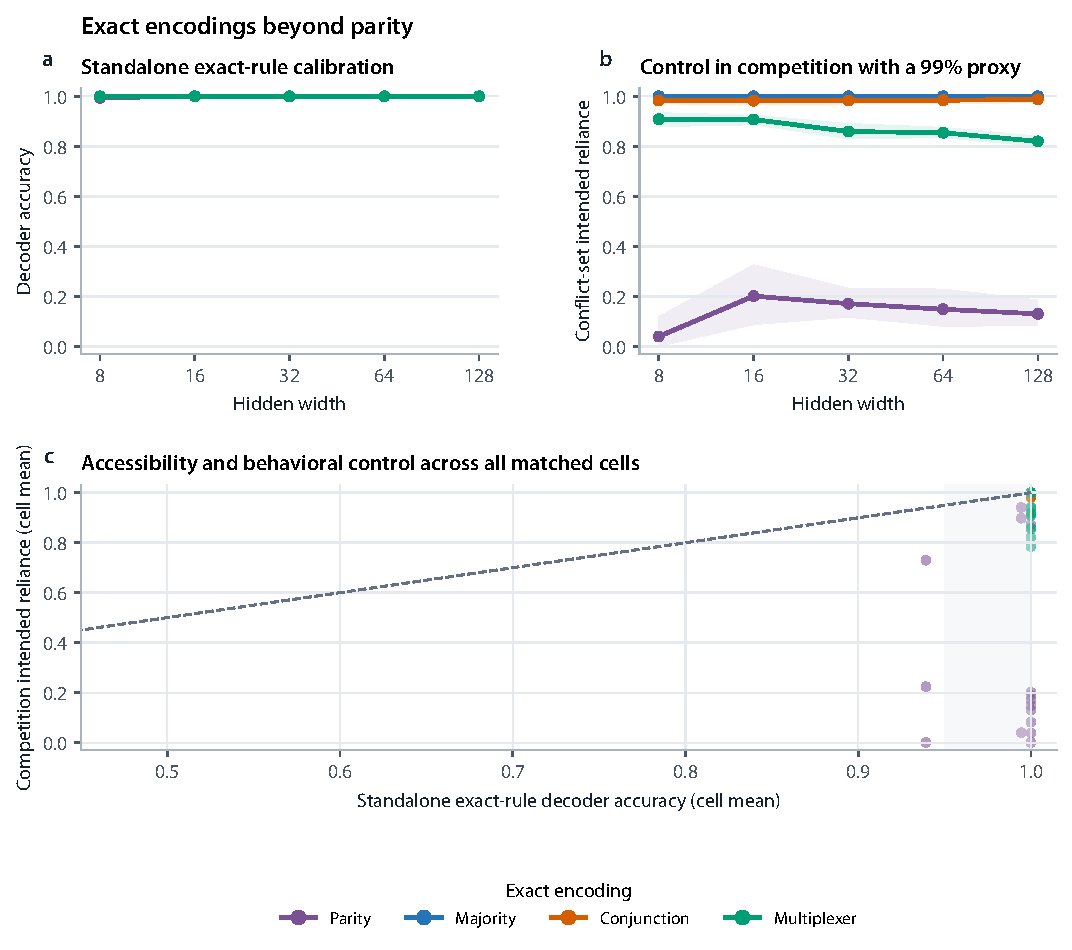
\includegraphics[width=\linewidth]{fig11_rule_families_followup.pdf}
  \caption{When exact rules with the same number of input channels compete against a 99\%-accurate proxy, outcomes range from proxy control to intended-rule control even though standalone calibration accuracy is near one. The comparison shows that channel count does not provide a portable measure of rule complexity; it does not establish a universal ordering of Boolean or natural-language goals.}
  \label{fig:lw-rules}
\end{figure}

\begin{figure}[!htbp]
  \centering
  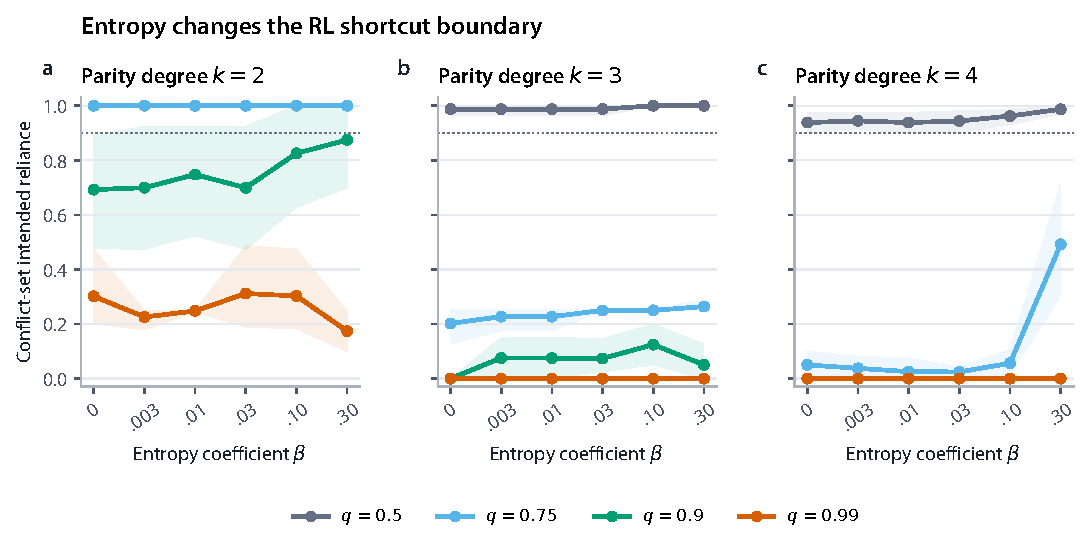
\includegraphics[width=\linewidth]{fig10_rl_entropy_followup.pdf}
  \caption{Across the tested entropy coefficients, the largest change in RL behavior occurs at $q=.75,k=4$, while no $q=.99$ setting becomes reliably controlled by the intended rule. The highlighted maximum is one of 24 setting-level comparisons, and the pre-specified threshold for the reference-setting mechanism analysis was not met.}
  \label{fig:lw-entropy}
\end{figure}

\begin{figure}[!htbp]
  \centering
  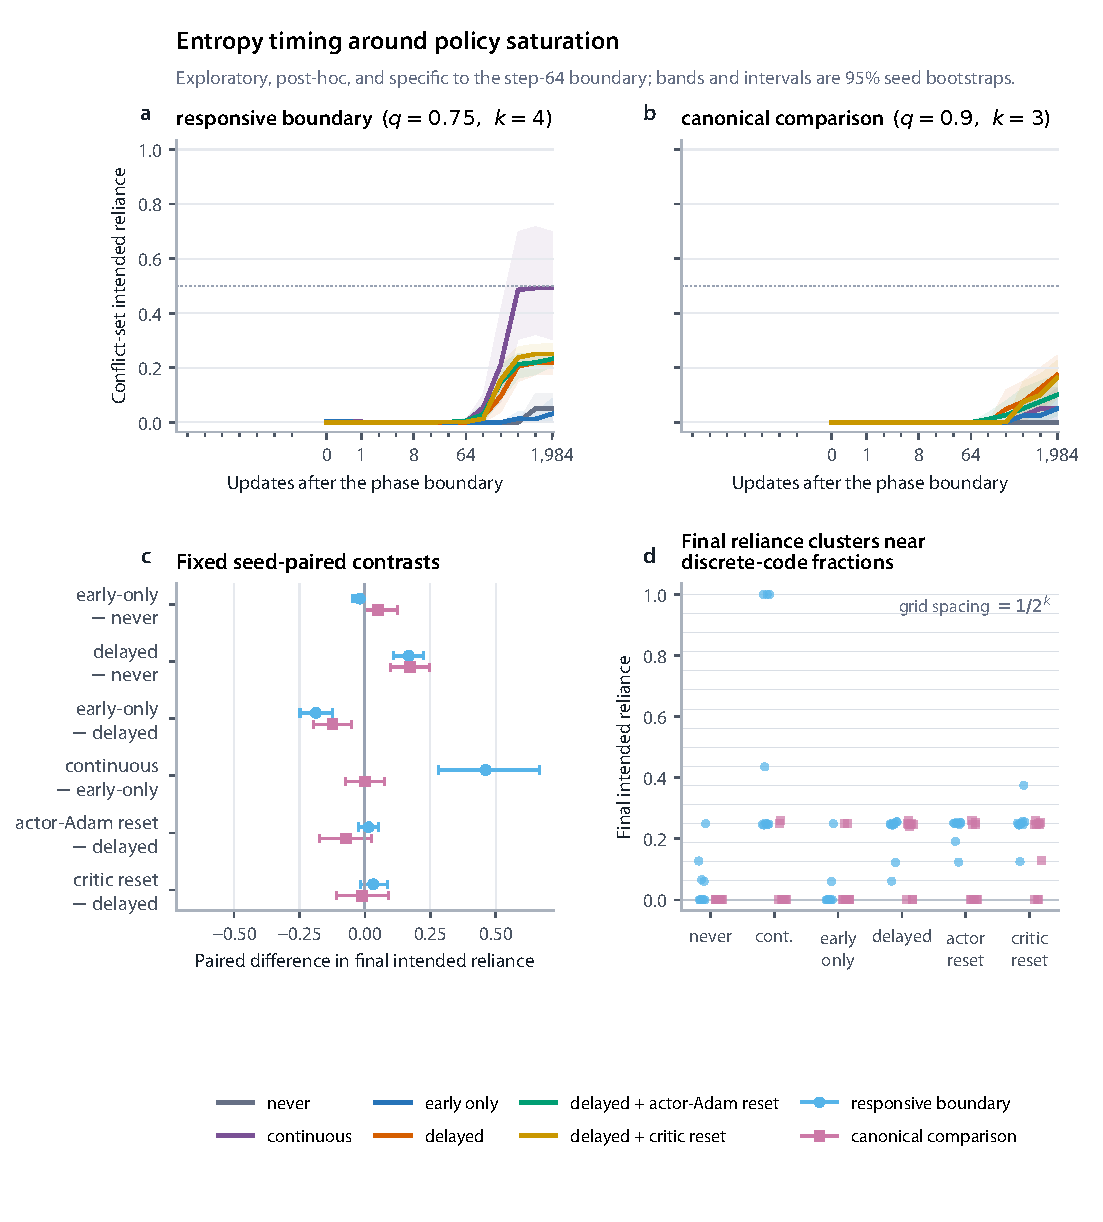
\includegraphics[width=\linewidth]{fig14_entropy_timing_exploratory.pdf}
  \caption{In the selected settings, introducing entropy regularization after update 64 partially increases intended-rule reliance. Endpoint values cluster near fractions of the finite parity truth table, which is consistent with nearly deterministic behavior on subsets of codewords rather than uniformly stochastic compromise. The schedule design and replay analysis are post-hoc.}
  \label{fig:lw-entropy-timing}
\end{figure}

\begin{figure}[!htbp]
  \centering
  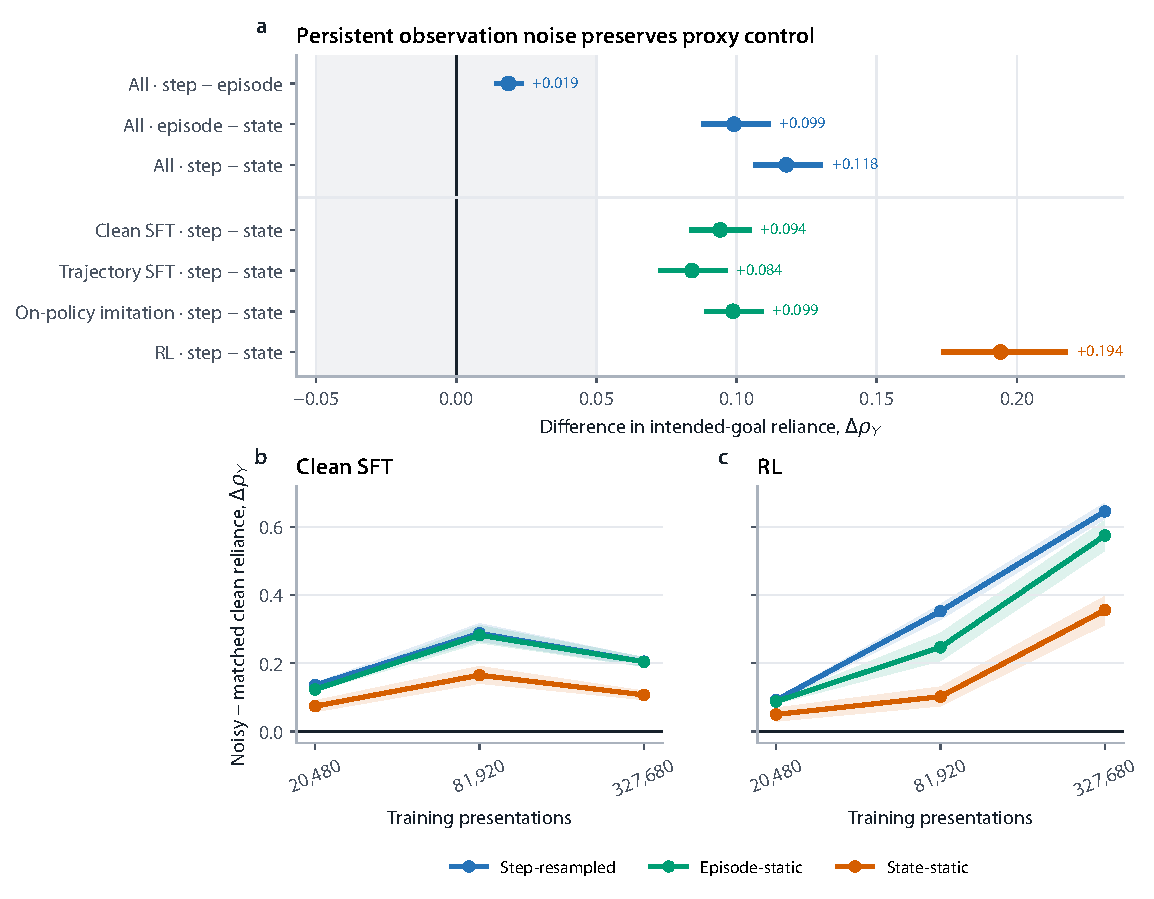
\includegraphics[width=\linewidth]{fig5_temporal_noise.pdf}
  \caption{The effect of proxy corruption depends on its temporal structure. Corruption tied to an underlying state preserves more proxy control than freshly sampled corruption, while the behavioral difference between fresh zero-mean corruption and the unperturbed condition grows over the tested sample and update schedule.}
  \label{fig:lw-noise}
\end{figure}

\begin{figure}[!htbp]
  \centering
  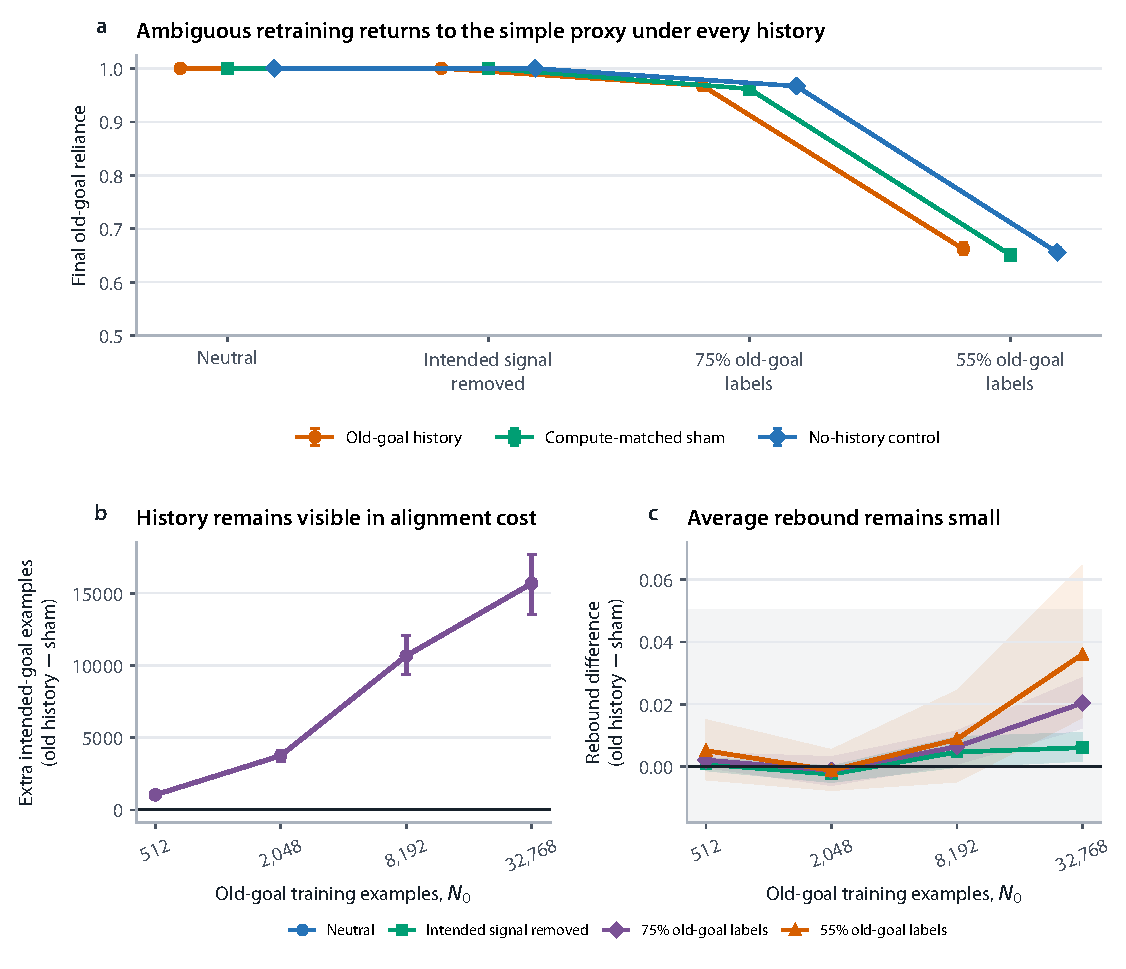
\includegraphics[width=\linewidth]{fig7_hysteresis.pdf}
  \caption{After ambiguous retraining, the endpoints for old-history, compute-matched random-label, and no-history conditions nearly overlap. Longer training on the old goal nevertheless requires substantially more intended-goal data to realign behavior.}
  \label{fig:lw-hysteresis}
\end{figure}

\begin{figure}[!htbp]
  \centering
  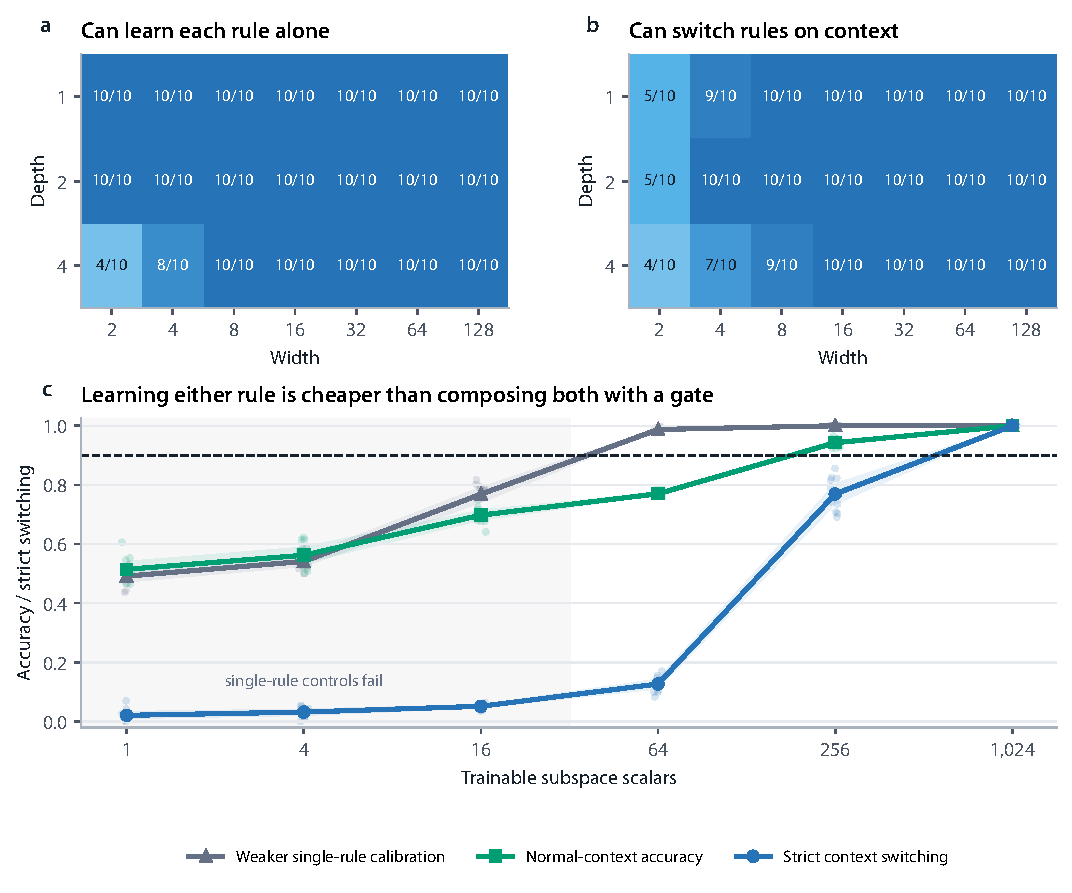
\includegraphics[width=\linewidth]{fig8_multiplicity_capacity.pdf}
  \caption{When only an intermediate number of parameters can change, separate calibration models learn both rules successfully, but the competition model does not yet switch reliably between them according to context.}
  \label{fig:lw-multiplicity}
\end{figure}

\begin{figure}[!htbp]
  \centering
  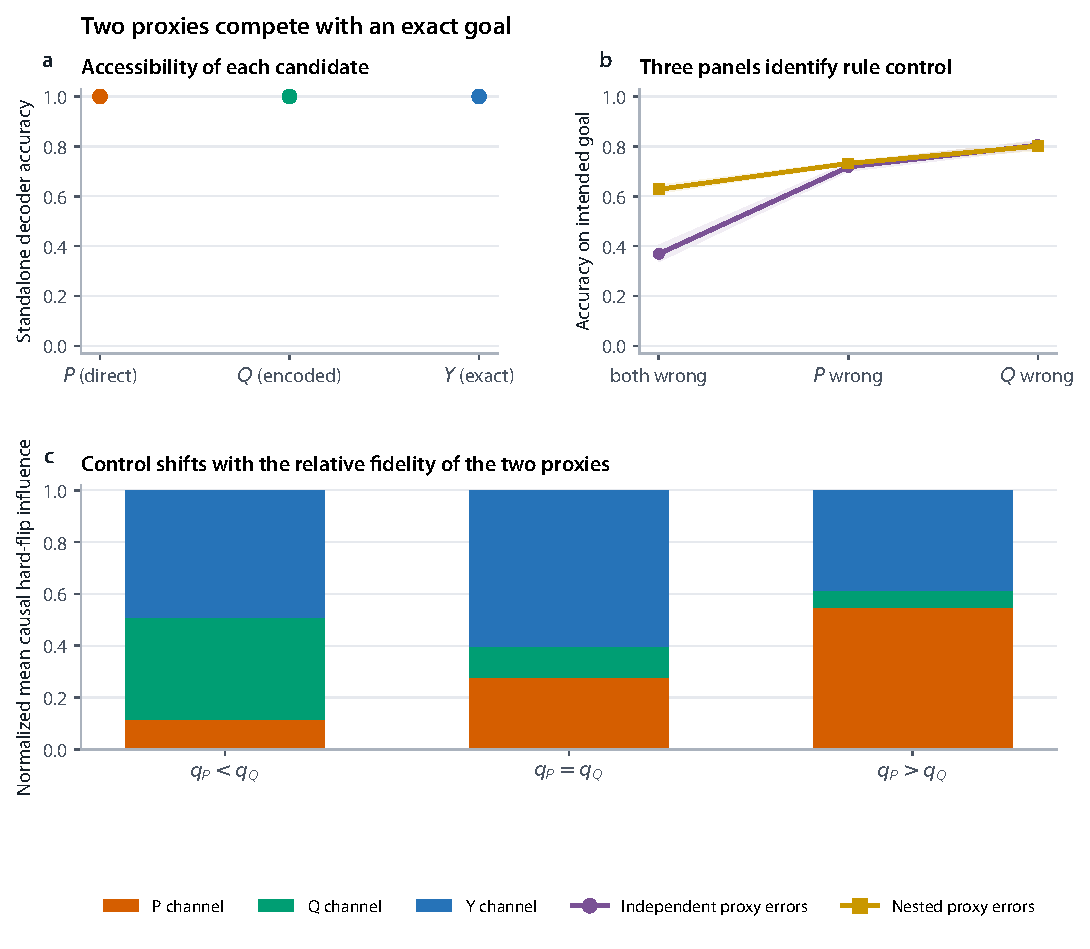
\includegraphics[width=\linewidth]{fig12_competing_goals_followup.pdf}
  \caption{Although each of the three candidate rules can be decoded when trained in isolation, which rule controls the competition model depends on proxy accuracy, encoding, model capacity, and the overlap between the proxies' errors. Some models also use context-dependent combinations of the rules.}
  \label{fig:lw-three-goals}
\end{figure}

\clearpage
\begin{landscape}
\begin{figure}[p]
  \centering
  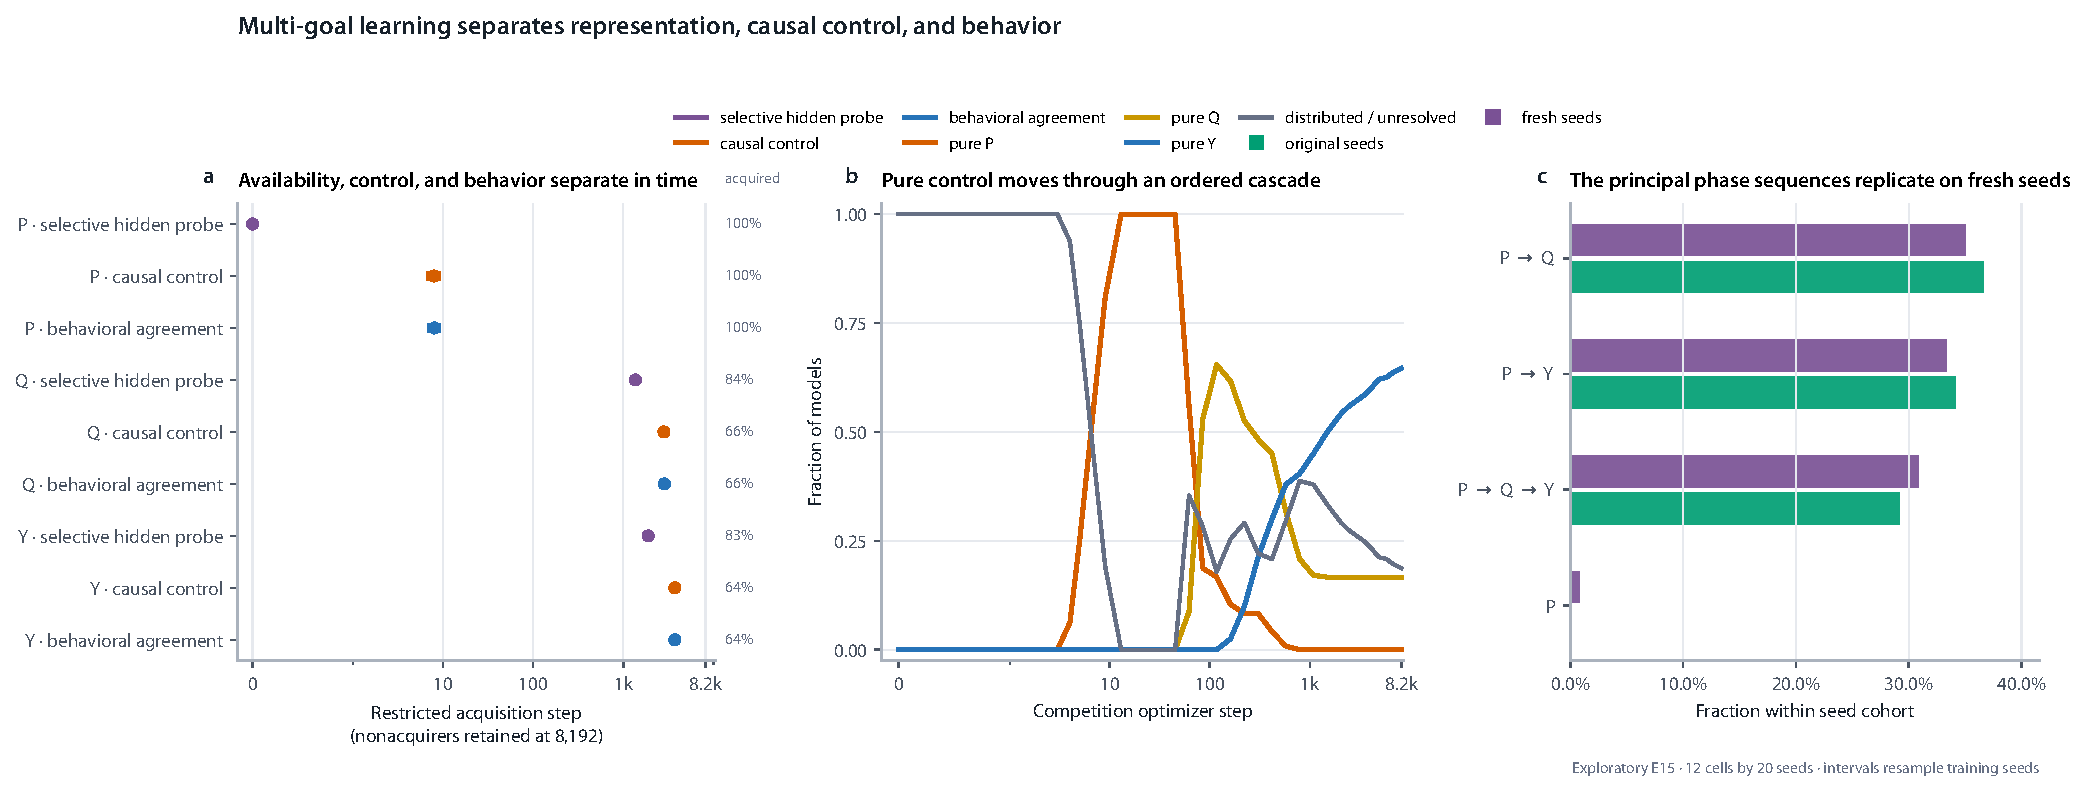
\includegraphics[width=0.86\linewidth,trim=0 18bp 0 25bp,clip]{fig15_multigoal_dynamics.pdf}
  \caption{Across the selected three-rule settings, all 240 training trajectories are controlled first by the direct proxy. Many later shift either to the encoded proxy or directly to the exact rule. Because these settings were selected after earlier results, the repeated learning sequences do not establish a universal law of training phases.}
  \label{fig:lw-multigoal-dynamics}
\end{figure}
\end{landscape}
\clearpage

\begin{landscape}
\begin{figure}[p]
  \centering
  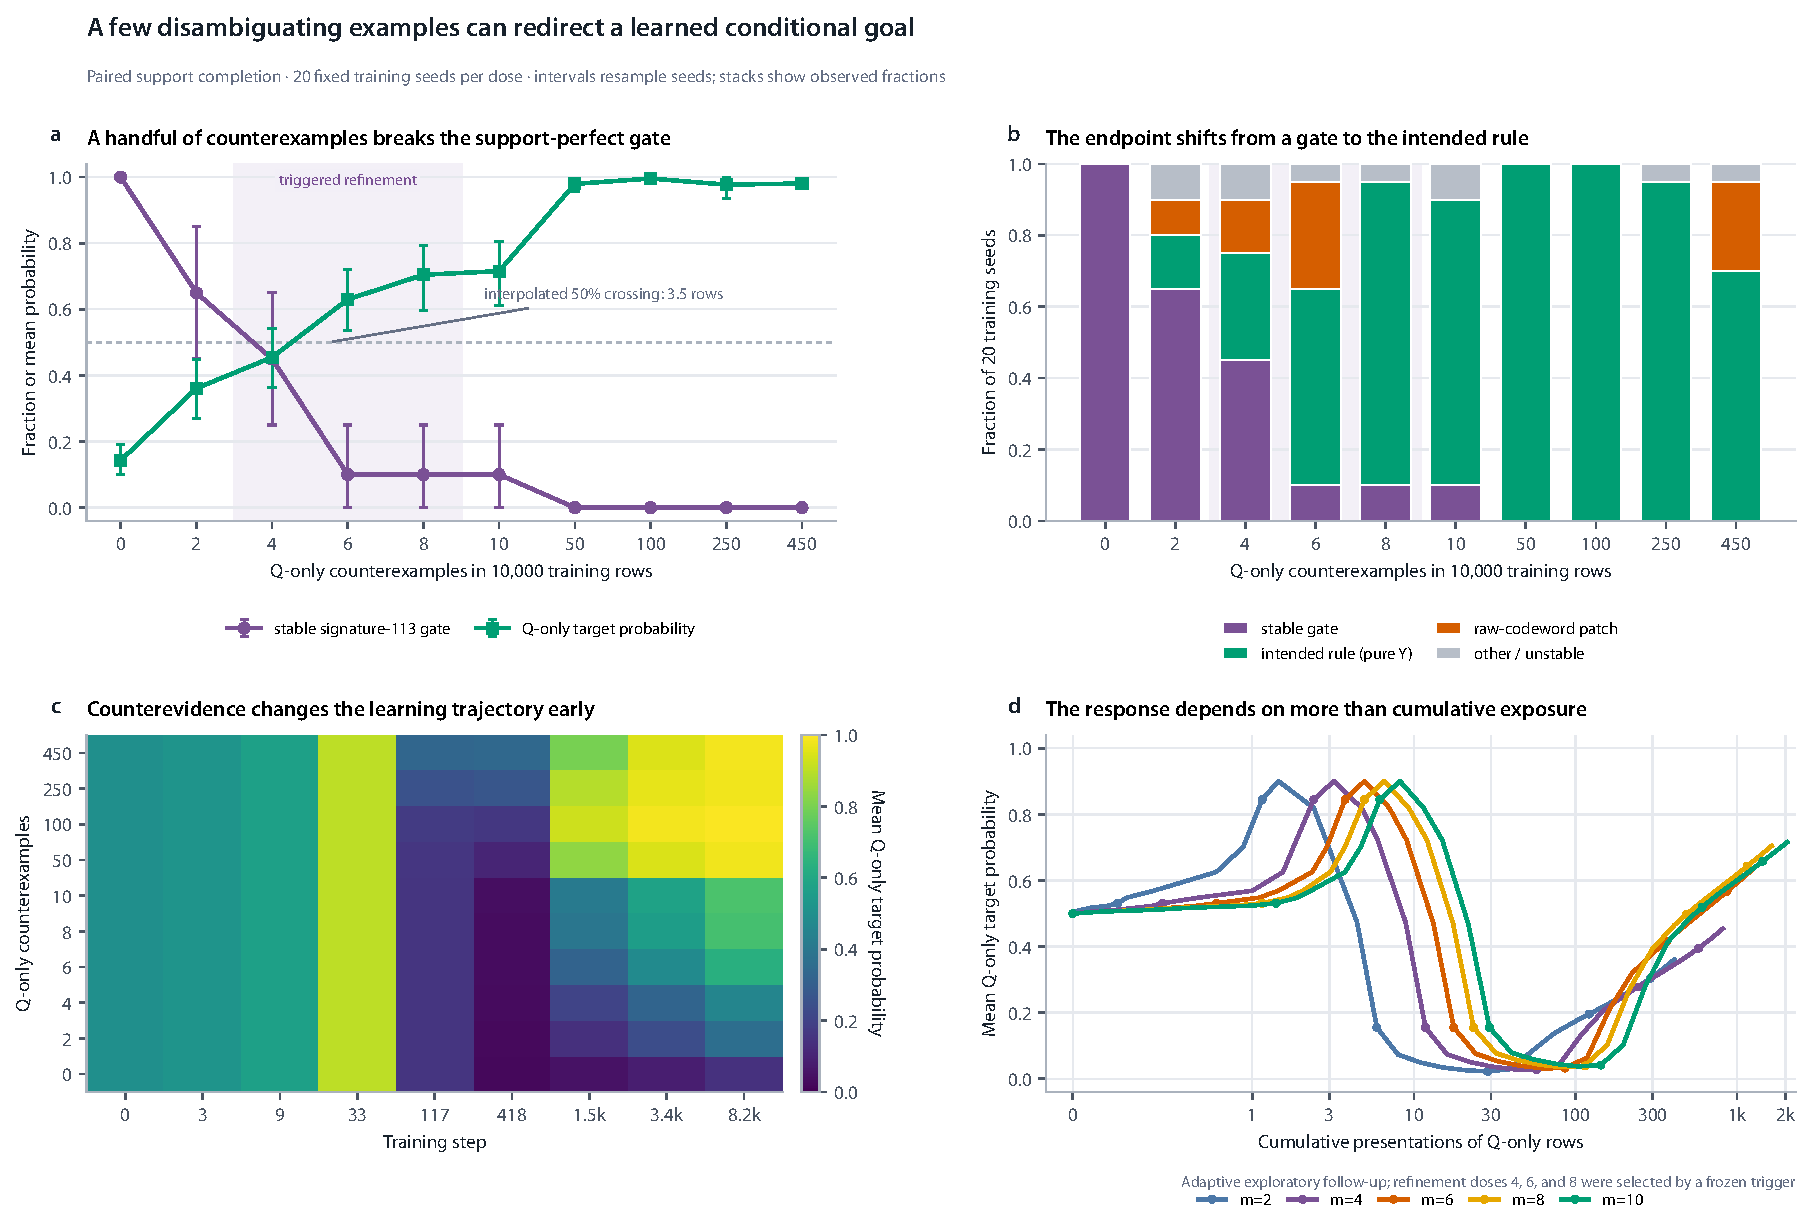
\includegraphics[width=0.78\linewidth]{fig16_support_completion.pdf}
  \caption{Adding a small number of previously absent examples in which only $Q$ is wrong changes which rule controls many models. These distinct examples are sampled repeatedly during training. Transfer tests and reversals at the seed level show that the result is not a uniform switch shared by every model.}
  \label{fig:lw-support}
\end{figure}
\end{landscape}
\clearpage

\begin{landscape}
\begin{figure}[p]
  \centering
  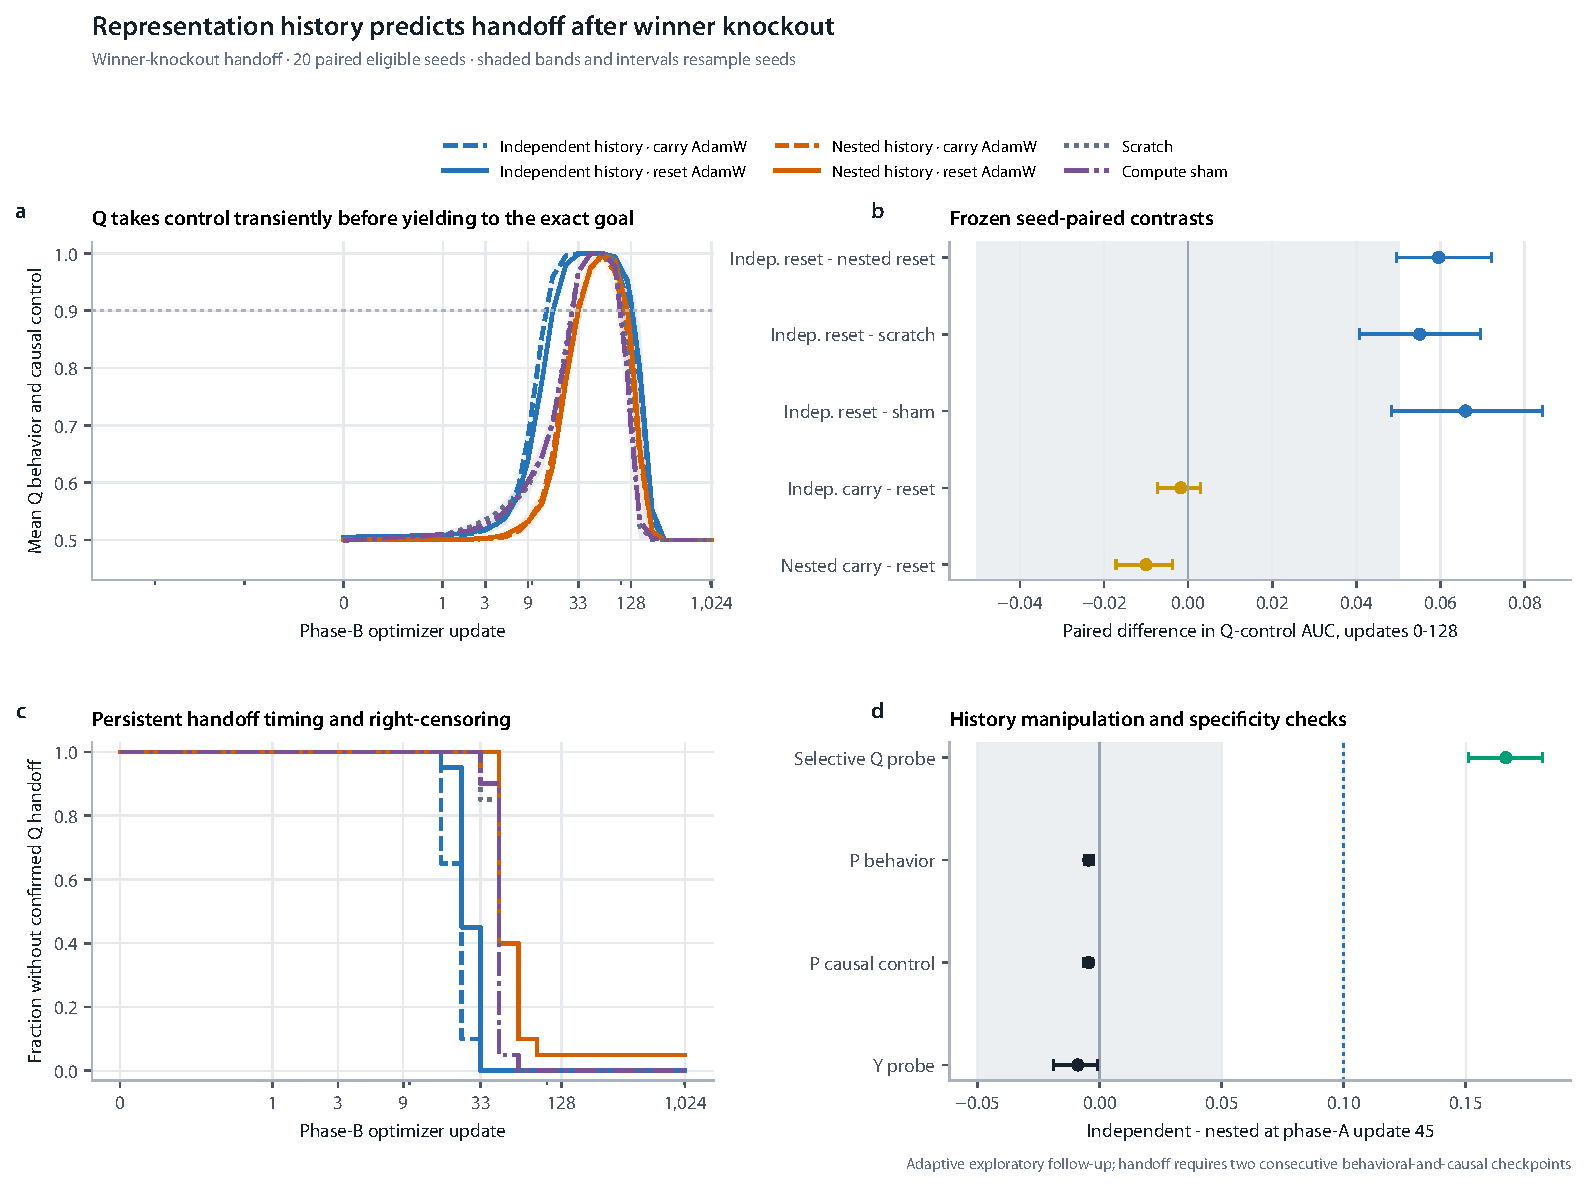
\includegraphics[width=0.76\linewidth]{fig17_winner_knockout.pdf}
  \caption{After the direct proxy becomes uninformative, models whose earlier proxy errors were independent shift to the encoded proxy sooner than models whose errors were nested. The histories also differ in how accurately $Q$ can be decoded and in which examples each proxy gets wrong. Every condition ultimately converges to the exact rule.}
  \label{fig:lw-knockout}
\end{figure}
\end{landscape}
\clearpage

\begin{figure}[!htbp]
  \centering
  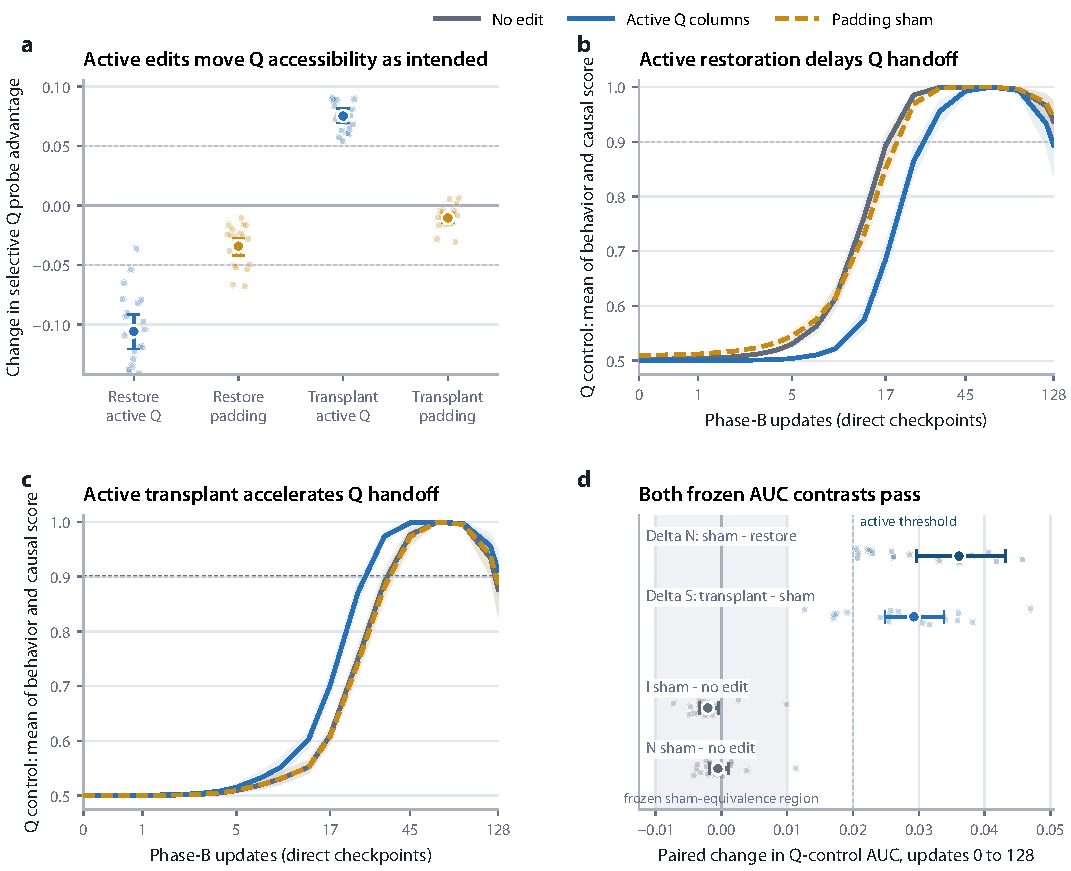
\includegraphics[width=\linewidth]{fig19_active_q_pathway.pdf}
  \caption{Restoring selected first-layer $Q$ weights to their initialization values delays early control by $Q$, while transplanting the corresponding weights from independent-error histories accelerates it. The two edits also change selective $Q$ decodability in opposite directions, whereas matched edits to padding weights have little effect. These interventions do not isolate a complete circuit.}
  \label{fig:lw-pathway}
\end{figure}

\begin{figure}[!htbp]
  \centering
  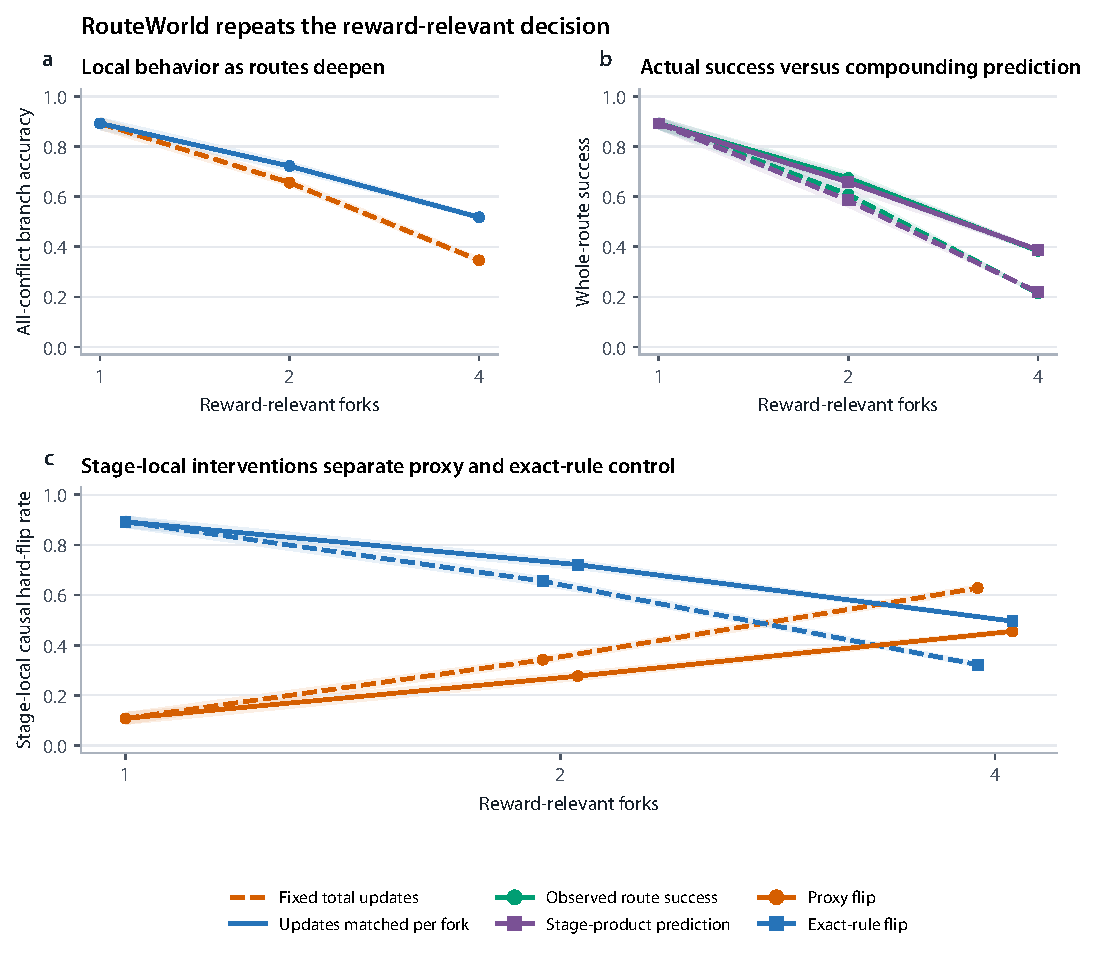
\includegraphics[width=\linewidth]{fig13_routeworld_followup.pdf}
  \caption{As RouteWorld depth increases, accuracy at each local fork decreases, and allocating more updates per fork recovers only part of this loss. The remaining local errors then reduce whole-route success. An exploratory calculation finds that multiplying stage-level accuracies closely predicts route success. Navigation between forks is scripted.}
  \label{fig:lw-routeworld}
\end{figure}

\FloatBarrier


\clearpage
\begingroup
\raggedright
\bibliography{references}
\endgroup

\end{document}
